% This is the University of Chicago Graham School Master of Science in Analytics
% template. Much of it is based on the Reed College LaTeX thesis template.
% Most of the work for the Reec College template was done by Sam Noble (SN),
% Later comments etc. by Ben Salzberg (BTS).
% Additional restructuring and APA support by Jess Youngberg (JY).
% Justin M. Shea (JMS) built on their good open source work.
% Your comments and suggestions are more than welcome:
% please email, them to justinshea@uchicago.edu.
%
% Any line that starts with a percent symbol is a comment.
% They won't show up in the document, and are useful for notes
% to yourself and explaining commands.
% Commenting also removes a line from the document;
% very handy for troubleshooting problems. -BTS
%%
%% Preamble
%%
% \documentclass{<something>} must begin each LaTeX document
% Added by JMS
\documentclass[12pt,oneside]{chicagocapstone}
% END of JMS add
% Packages are extensions to the basic LaTeX functions. Whatever you
% want to typeset, there is probably a package out there for it.
% Check out CTAN to see: http://www.ctan.org/
%%
\usepackage{graphicx,latexsym}
\usepackage{amsmath}
\usepackage{amssymb,amsthm}
\usepackage{longtable,booktabs,setspace}
\usepackage[hyphens]{url}
% Added by CII
\usepackage{hyperref}
\usepackage{lmodern}
\usepackage{float}
\floatplacement{figure}{H}
% End of CII addition
\usepackage{rotating}


% Added by CII (Thanks, Hadley!)
% Use ref for internal links
\renewcommand{\hyperref}[2][???]{\autoref{#1}}
\def\chapterautorefname{Chapter}
\def\sectionautorefname{Section}
\def\subsectionautorefname{Subsection}
% End of CII addition

% Added by CII
\usepackage{caption}
\captionsetup{width=5in}
% End of CII addition

% Added by JMS
\usepackage{mathptmx} % Times New Roman fonts
% End of add by JMS

% Syntax highlighting #22

% To pass between YAML and LaTeX the dollar signs are added by CII
\title{Forecasting Coca-Cola Bag Orders Using Social Media}
\author{Elijah Ampo, Ruohan Zhou, and Yingkun Zhu}
\date{May, 2019} % The month and year that you submit your FINAL draft)
\division{Graham School}
\advisor{Arnab Bose}
\institution{University of Chicago}
\degree{Master of Science in Analytics}
\altadvisor{Dr.~Sema Barlas}
% End of CII addition

\department{Continuing Liberal and Professional Studies}

% Added by CII
%%% Copied from knitr
%% maxwidth is the original width if it's less than linewidth
%% otherwise use linewidth (to make sure the graphics do not exceed the margin)
\makeatletter
\def\maxwidth{ %
  \ifdim\Gin@nat@width>\linewidth
    \linewidth
  \else
    \Gin@nat@width
  \fi
}
\makeatother

\renewcommand{\contentsname}{Table of Contents}
% End of CII addition

\setlength{\parskip}{0pt}

% Added by CII
  %\setlength{\parskip}{\baselineskip}
  \usepackage[parfill]{parskip}

\providecommand{\tightlist}{%
  \setlength{\itemsep}{0pt}\setlength{\parskip}{0pt}}


\Abstract{
Scholle IPN is a global manufacturing company that has experienced variability in their sales forecasts. In this project, we demonstrate how Scholle IPN can leverage social media data to predict orders from their clients. We introduce dimension reduction methods to account for the high dimensional nature of social media data. In addition, an ensemble model approach to sales forecasting is used to generate the best sales forecasting model.

\bigskip 
\bigskip
\bigskip

\textbf{Keywords}: Time Series, Machine Learning, sARIMA, Regression with ARIMA Errors, XGBoost, Long Short-Term Memory (LSTM), Ensemble, Social Media, Linear Regression.

\bigskip 
\bigskip
\bigskip
}

% Added by JMS
\Executive{
Manufacturing companies need to forecast the demand of their products ahead of time, and failing to predict the future demand can result in over-producing, loss of business opportunities, etc. In an era where social media dominates people's life, and data analytics are growing more and more powerful on generating actionable business insights, Scholle IPN tasks us to test if social media brings any predictive power to forecast the future Coca-Cola bag sales. In this project, we examine whether or not people's discussion and engagement on social media have any impact on the consumption of the Coke product in real life.

In order to achieve that, we start with collecting external data from social media, and combine with the internal data provided by Scholle IPN. After preliminary exploratory analysis, we build traditional Regression with ARIMA errors model, then more advanced machine learning models, namely, XGBoost and LSTM RNN. XGBoost using the differenced social media variables returns the best predictions (lowest sMAPE score) among all the individual models while still has a decent level of interpretability. Following individual models and their results, we stack these individual models together and create three ensemble models - mean average, linear regression, and random forest. Linear regression ensemble model achieves is the most stable, with the lowest error score.

Key findings from this project including the following:
\begin{enumerate}
\def\labelenumi{\arabic{enumi}.}
\tightlist
\item
  Different social media variables have different importances when modeling. Surprisingly, Pepsi and Taco Bell lagged variables showed the most importance among the predictors according to our XGBoost model feature importance.
\item
  Ensemble modeling is a great way to bring the individual models together, and establish a better model with stronger predictive capacity. We observe the forecasts of the ensemble model to be the best among all indidivual models. Furthermore, ensembling the models from all Scholle IPN capstone teams produced the best overall model.
\item
  Reducing the dimensionality when handling a large number of features improves the predictive accuracy; Cross Correlation check, Principal Component Analysis are vital steps for modeling.
\end{enumerate}
We conclude that Scholle IPN should continue monitoring social media conversations, and follow our practice of adding the social media variables to the internal historical sales data. For future work, we recommend an examination of the year-to-year comparison between the forecasting bag sales with the actual bag sales.\\
}
% End of JMS add

\Acknowledgements{

}

\Dedication{

}

\Preface{

}


% End of CII addition
%%
%% End Preamble
%%
%
\begin{document}

% Everything below added by CII
  \maketitle

\frontmatter % this stuff will be roman-numbered
\pagestyle{empty} % this removes page numbers from the frontmatter


%% Reorganized by JMS
  \begin{abstract}
    Scholle IPN is a global manufacturing company that has experienced variability in their sales forecasts. In this project, we demonstrate how Scholle IPN can leverage social media data to predict orders from their clients. We introduce dimension reduction methods to account for the high dimensional nature of social media data. In addition, an ensemble model approach to sales forecasting is used to generate the best sales forecasting model.
    
    \bigskip 
    \bigskip
    \bigskip
    
    \textbf{Keywords}: Time Series, Machine Learning, sARIMA, Regression with ARIMA Errors, XGBoost, Long Short-Term Memory (LSTM), Ensemble, Social Media, Linear Regression.
    
    \bigskip 
    \bigskip
    \bigskip
  \end{abstract}
 % Added by JMS
  \begin{executive}
    Manufacturing companies need to forecast the demand of their products ahead of time, and failing to predict the future demand can result in over-producing, loss of business opportunities, etc. In an era where social media dominates people's life, and data analytics are growing more and more powerful on generating actionable business insights, Scholle IPN tasks us to test if social media brings any predictive power to forecast the future Coca-Cola bag sales. In this project, we examine whether or not people's discussion and engagement on social media have any impact on the consumption of the Coke product in real life.
    
    In order to achieve that, we start with collecting external data from social media, and combine with the internal data provided by Scholle IPN. After preliminary exploratory analysis, we build traditional Regression with ARIMA errors model, then more advanced machine learning models, namely, XGBoost and LSTM RNN. XGBoost using the differenced social media variables returns the best predictions (lowest sMAPE score) among all the individual models while still has a decent level of interpretability. Following individual models and their results, we stack these individual models together and create three ensemble models - mean average, linear regression, and random forest. Linear regression ensemble model achieves is the most stable, with the lowest error score.
    
    Key findings from this project including the following:
    \begin{enumerate}
    \def\labelenumi{\arabic{enumi}.}
    \tightlist
    \item
      Different social media variables have different importances when modeling. Surprisingly, Pepsi and Taco Bell lagged variables showed the most importance among the predictors according to our XGBoost model feature importance.
    \item
      Ensemble modeling is a great way to bring the individual models together, and establish a better model with stronger predictive capacity. We observe the forecasts of the ensemble model to be the best among all indidivual models. Furthermore, ensembling the models from all Scholle IPN capstone teams produced the best overall model.
    \item
      Reducing the dimensionality when handling a large number of features improves the predictive accuracy; Cross Correlation check, Principal Component Analysis are vital steps for modeling.
    \end{enumerate}
    We conclude that Scholle IPN should continue monitoring social media conversations, and follow our practice of adding the social media variables to the internal historical sales data. For future work, we recommend an examination of the year-to-year comparison between the forecasting bag sales with the actual bag sales.\\
  \end{executive}
 % End of JMS




  \hypersetup{linkcolor=black}
  \setcounter{tocdepth}{2}
  \tableofcontents

  \listoffigures

  \listoftables

%% END of Reorganization by JMS

\mainmatter % here the regular arabic numbering starts
\pagestyle{fancyplain} % turns page numbering back on

\hypertarget{introduction}{%
\chapter*{Introduction}\label{introduction}}
\addcontentsline{toc}{chapter}{Introduction}

Scholle IPN is a global manufacturing company based in Northlake, IL, with products focused primarily in bag-in-box packaging. The company is a pioneer in its industry by implementing a combination of qualitative observations and quantitative analyses in forecasting their products' sales. However, variability in these sales forecasts present challenges for Scholle IPN in raw material preparation, operational efficiency, and asset management.

\hypertarget{problem-statement}{%
\section*{Problem Statement}\label{problem-statement}}
\addcontentsline{toc}{section}{Problem Statement}

In this project, we provide a forecasting solution to Scholle IPN using social media data. This project primarily focuses on one of Scholle IPN's main clients, Coca-Cola. Coca-Cola uses Scholle IPN's state-of-the art bags to store beverage products at quick service restaurant (QSR) partners worldwide. Since 2014, Coca-Cola has accounted for 95.68\% of Scholle's syrup-related bag order shipments, so inaccurate forecasts of future orders could result in operational inefficiencies. Minimizing these operational inefficiencies is important to maintain Scholle's partnership with Coca-Cola. In order to solve this business problem, we examine whether we can substantially improve Scholle IPN's Coca-Cola demand forecasts by using social media as the primary variable.

\hypertarget{research-purpose}{%
\section*{Research Purpose}\label{research-purpose}}
\addcontentsline{toc}{section}{Research Purpose}

The purpose of this research is to forecast Coca-Cola bag orders by utilizing social media data. When customer express their opinions in social media, businesses like Scholle IPN can gain valuable insights that can inform business decisions. For example, if a McDonald's promotion is generating discussion posts online, then Scholle IPN can potentially expect an increase in bag orders from Coca-Cola. In order to make these online discussions actionable, we must first take into account additional considerations. First, since social media posts are usually in the form of text, we explore methods to convert text to numerical data. Second, we explore different ways to reduce the dimension of social media variables to account for its high dimensionality. And finally, we use these social media variables to forecast Coca-Cola bag orders using an ensemble approach. Below is a list of research objectives for this project:
\begin{itemize}
\tightlist
\item
  Convert text-based social media data to numerical data using natural language processing.
\item
  Reduce the dimension of social media variables using different methods.
\item
  Forecast Coca-Cola bag orders using an ensemble approach.
\end{itemize}
\hypertarget{variables-and-scope}{%
\section*{Variables and Scope}\label{variables-and-scope}}
\addcontentsline{toc}{section}{Variables and Scope}

The scope of this forecasting project is limited to predicting the future monthly bag orders for Coca-Cola in the United States and Canada. All variables will be aggregated or averaged at the monthly level. The forecasting window for this project will be 18 months for all models to accommodate Scholle's business needs. The main social media variables used to predict Coca-Cola bag orders were collected from Twitter and Google Trends. For Twitter, we focus our project on the following variables: tweet text, number of likes, number of retweets, and number of replies. For Google Trends, monthly trend values for selected topics are extracted at the monthly level. Additional data retrieval rules are applied to ensure that Twitter and Google Trends data are from the United States and Canada (see Appendix A).

\hypertarget{background}{%
\chapter*{Background}\label{background}}
\addcontentsline{toc}{chapter}{Background}

\hypertarget{social-media-variables}{%
\section*{Social Media Variables}\label{social-media-variables}}
\addcontentsline{toc}{section}{Social Media Variables}

For this forecasting project, we focus on collecting social media data on relevant topics. These relevant topics are Coca-Cola, Pepsi, McDonald's, Taco Bell, and ``jobs''. Coca-Cola is selected because it is their product's demand that Scholle IPN is interested in forecasting. Pepsi is selected due to its position as the main competitor for Coca-Cola. Meanwhile, McDonald's and Taco Bell are chosen because they are the top quick service restaurant partners for Coca-Cola and Pepsi based on 2018 annual sales revenue. The topic `jobs' is selected to gather job-related tweets intended to capture economic activity in the United States and Canada. Relationships between social media activity on these topics and the quantity of Coca-Cola bag ordered can be useful information for our forecasting models.
Twitter data is a combination of user-level tweets and company-level tweets, while Google Trend data is monthly trend value for our selected terms. User-level tweets are Twitter posts from regular online consumers tweeting about Coca-Cola, Pepsi, McDonald's, Taco Bell, and ``jobs.'' Company-level tweets are Twitter posts by the official Twitter accounts of Coca-Cola, Pepsi, McDonald's, and Taco Bell. Meanwhile, Google Trends is a popularity measure for Coca-Cola and other relevant terms based on their search frequency over time.

\hypertarget{sentiment-analysis}{%
\section*{Sentiment Analysis}\label{sentiment-analysis}}
\addcontentsline{toc}{section}{Sentiment Analysis}

One method of quantifying text-based social media data for our forecasting models is by implementing sentiment analysis. This is a technique in natural language processing that we use for each tweet to generate a numerical value signifying whether consumers have a positive or negative outlook on Coca-Cola, Pepsi, McDonald's, Taco Bell, or `jobs'. We then average sentiment scores by month for each relevant term, and use this as an additional predictor to forecast Coca-Cola bag orders. For this project, we only calculate sentiment scores for user-generated tweets because we assume that tweets generated by the official company accounts are positively biased towards their own brand. Prior to conducting sentiment analysis, text processing steps must be conducted on tweets. The following steps were conducted on the tweets:
\begin{itemize}
\tightlist
\item
  Remove stop words on tweets
\item
  Tokenize tweets
\item
  Lemmatize tweets
\end{itemize}
The R package sentimentR was used to calculate sentiment scores for each tweet. This package takes into account additional information such as valence shifters and de-amplifiers resulting in a more accurate sentiment score (see Appendix A). The sentiment scores for each selected term's collective tweets per month is averaged at the monthly level to generate the monthly average sentiment variable.

\hypertarget{stationarity-and-differencing}{%
\section*{Stationarity and Differencing}\label{stationarity-and-differencing}}
\addcontentsline{toc}{section}{Stationarity and Differencing}

An important step to consider when forecasting is to remove trends and seasonality from variables in order to make it stationary. When time series data is stationary, it displays a stable mean and stable variance over time (Hyndman, 2018). This means that it is less likely to produce spurious relationships and misleading results. Statistical tests (KPSS test) (Kwiatkowski, 1992) are conducted on each variable to determine its level of stationarity (Hyndman, 1992). After testing, it was determined that the dependent variable, monthly quantity of Coca-Cola bag orders, is stationary. This means that this variable requires no further transformations. However, the independent variables show varying results and require additional processing. One way of transforming time series data to become stationary is the method of differencing. Differencing is the method of subtracting the value of the current time step from the value of previous time step(s). This method was applied to all social media variables to ensure that they were all stationary. The visual below demonstrates how the method of differencing is able to remove trends from the monthly total user tweets. The top half of the visual are time plots of the pre-differenced variables, while the bottom are time plots of the differenced variables.
\begin{figure}

{\centering 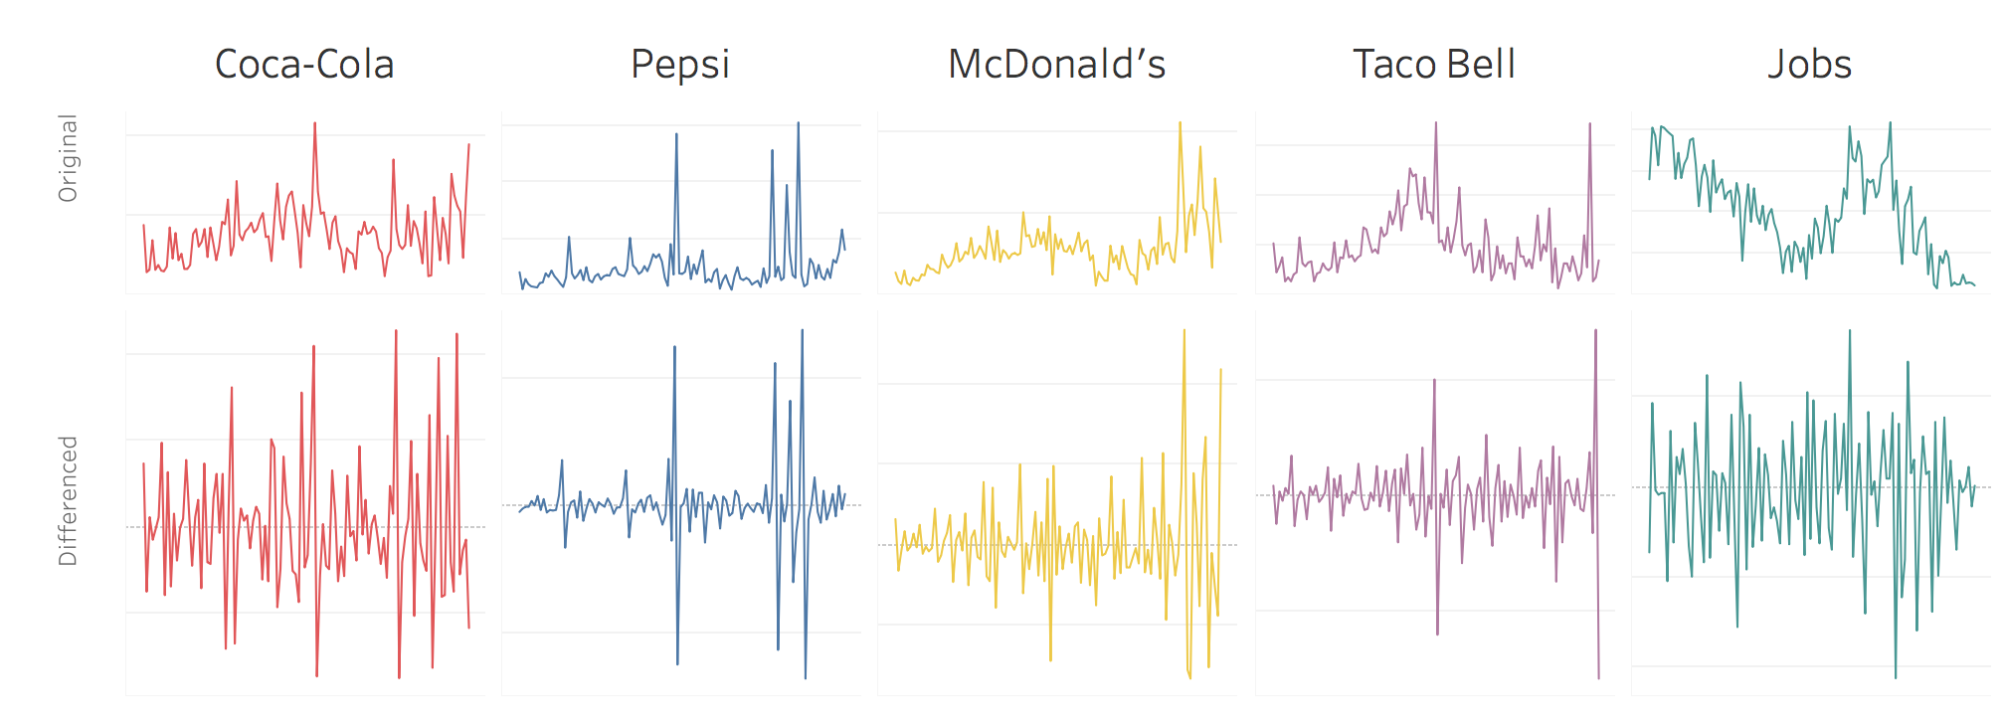
\includegraphics[width=200px,angle = 0, scale=2.1]{figure/differencing} 

}

\caption{Differenced social media variables}\label{fig:differencing}
\end{figure}
\hypertarget{dimension-reduction}{%
\section*{Dimension Reduction}\label{dimension-reduction}}
\addcontentsline{toc}{section}{Dimension Reduction}

When building forecasting models, it is important to be aware of the level of complexity of these models. In this project, we collect Twitter data with over a hundred features for a single tweet (tweet text, user profile data, etc.). Using all of these variables will make our forecasting models highly complex and likely result in poor predictions. Fortunately, the scope of this project limits tweet information to only a tweet's text, number of likes, number of retweets, and number of replies. However, the complexity of this project (relevant topics, social media data type, social media source) still leaves us with 46 total independent variables per observation (see Data section). We will use two main approaches in this project to further reduce our social media variable's dimensions.

\hypertarget{method-a---principal-component-analysis}{%
\subsubsection*{Method A - Principal Component Analysis}\label{method-a---principal-component-analysis}}
\addcontentsline{toc}{subsubsection}{Method A - Principal Component Analysis}

The first method we will use to reduce the dimensionality of our social media variables is principal component analysis (PCA). PCA uses an orthogonal transformation of our variables into linearly uncorrelated variables called principal components (Kambhatla, 1997). The main idea is that the majority of the variance explained will be concentrated on a limited number of principal components. This allows us to discard the principal component variables that provide little additional information. This approach further reduces the overall dimension of our original set of variables. When performing this technique with our social media variables, we are able to observe the ``elbow feature'' at number of principal component (n) = 7 . This tells us that only the first seven principal components is required to explain most of the total variance (97\%) of our variables. By using PCA, we are able to reduce our overall social media variables from 46 to 7.
\begin{figure}

{\centering 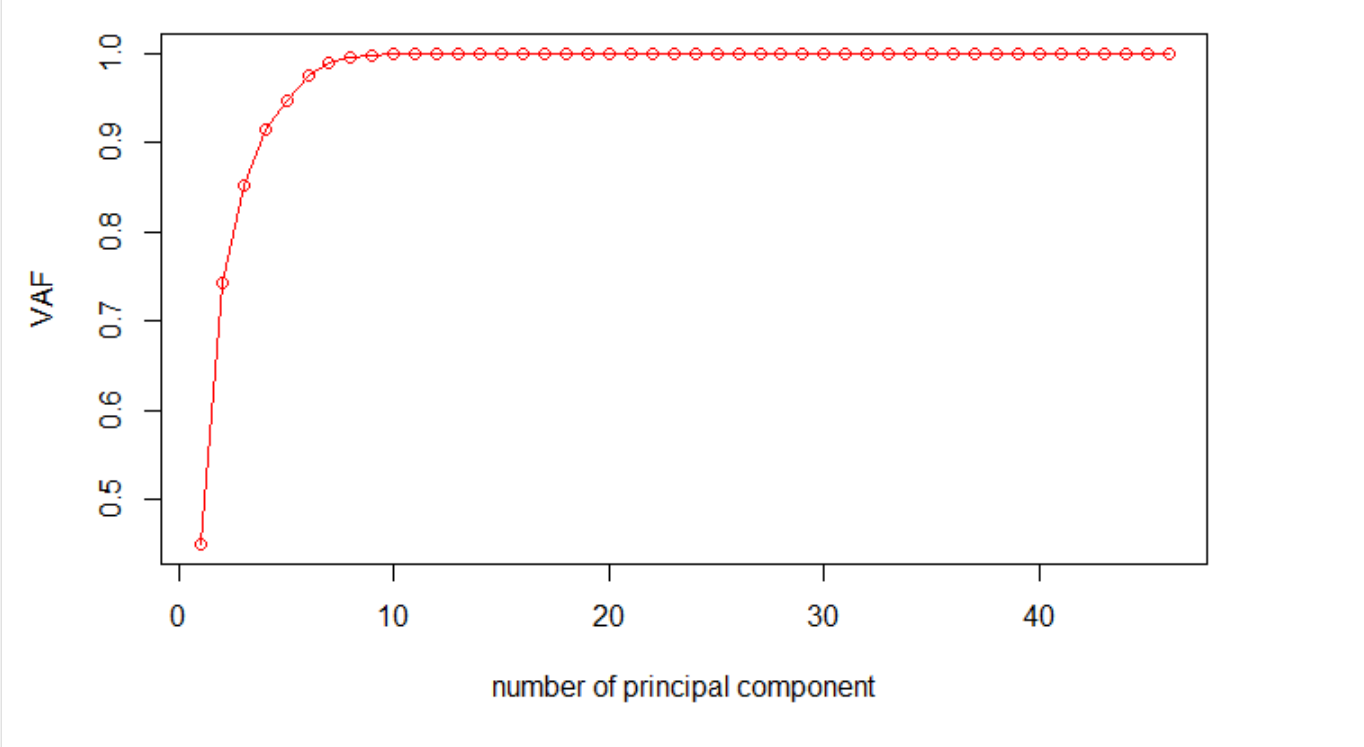
\includegraphics[width=200px,angle = 0, scale=2.1]{figure/pca} 

}

\caption{Variable Explained vs. Principal Components Plot}\label{fig:pca}
\end{figure}
\hypertarget{method-b---cross-correlation}{%
\subsubsection*{Method B - Cross Correlation}\label{method-b---cross-correlation}}
\addcontentsline{toc}{subsubsection}{Method B - Cross Correlation}

The second method we employ to reduce our total features is by testing our independent variables for cross correlation with the dependent variable (Brockwell, 1991). Mainly, this approach will inform us how many months in advance a social media variable can lead to an increase or decrease in Coca-Cola bag orders. For example, consider when a social media variable was found to be significantly positively correlated with Coca-Cola bag orders at lag t-1. If this social media variable has a positive value for the current month, then an increase in Coca-Cola bag orders can be expected the following month. In this project, we check for cross correlation on each independent variable up to six months prior (t-6). We will do this on the original variables as well as the principal component variables. Using the cross correlation approach, we identified eight lags from the social media variables that were cross correlated with Coca-Cola bag orders. Below is a table of these social media variables with their specified lags listed.
\begin{longtable}[]{@{}cc@{}}
\caption{\label{tab:inher} Social Media Variables with Specified Lags}\tabularnewline
\toprule
\begin{minipage}[b]{0.44\columnwidth}\centering
Social Media Variable\strut
\end{minipage} & \begin{minipage}[b]{0.39\columnwidth}\centering
Significant Lag\strut
\end{minipage}\tabularnewline
\midrule
\endfirsthead
\toprule
\begin{minipage}[b]{0.44\columnwidth}\centering
Social Media Variable\strut
\end{minipage} & \begin{minipage}[b]{0.39\columnwidth}\centering
Significant Lag\strut
\end{minipage}\tabularnewline
\midrule
\endhead
\begin{minipage}[t]{0.44\columnwidth}\centering
Coca-Cola Account tweets\strut
\end{minipage} & \begin{minipage}[t]{0.39\columnwidth}\centering
t-1\strut
\end{minipage}\tabularnewline
\begin{minipage}[t]{0.44\columnwidth}\centering
Taco Bell Account tweets\strut
\end{minipage} & \begin{minipage}[t]{0.39\columnwidth}\centering
t-1\strut
\end{minipage}\tabularnewline
\begin{minipage}[t]{0.44\columnwidth}\centering
Job Google Trend\strut
\end{minipage} & \begin{minipage}[t]{0.39\columnwidth}\centering
t-2\strut
\end{minipage}\tabularnewline
\begin{minipage}[t]{0.44\columnwidth}\centering
McDonald's Google Trend\strut
\end{minipage} & \begin{minipage}[t]{0.39\columnwidth}\centering
t-2\strut
\end{minipage}\tabularnewline
\begin{minipage}[t]{0.44\columnwidth}\centering
McDonald's Account replies\strut
\end{minipage} & \begin{minipage}[t]{0.39\columnwidth}\centering
t-5\strut
\end{minipage}\tabularnewline
\begin{minipage}[t]{0.44\columnwidth}\centering
Taco Bell Google Trend\strut
\end{minipage} & \begin{minipage}[t]{0.39\columnwidth}\centering
t-5\strut
\end{minipage}\tabularnewline
\begin{minipage}[t]{0.44\columnwidth}\centering
McDonald's Google Trend\strut
\end{minipage} & \begin{minipage}[t]{0.39\columnwidth}\centering
t-5\strut
\end{minipage}\tabularnewline
\begin{minipage}[t]{0.44\columnwidth}\centering
Pepsi Account tweets\strut
\end{minipage} & \begin{minipage}[t]{0.39\columnwidth}\centering
t-6\strut
\end{minipage}\tabularnewline
\bottomrule
\end{longtable}
In addition, we identified seven lags from principal components that are cross correlated with Coca-Cola bag orders. Below is a table of these principal components with their specified lags listed.
\begin{longtable}[]{@{}cc@{}}
\caption{\label{tab:inher} Principal Components with Specified Lags}\tabularnewline
\toprule
\begin{minipage}[b]{0.34\columnwidth}\centering
Principal Component\strut
\end{minipage} & \begin{minipage}[b]{0.44\columnwidth}\centering
Significant Lag\strut
\end{minipage}\tabularnewline
\midrule
\endfirsthead
\toprule
\begin{minipage}[b]{0.34\columnwidth}\centering
Principal Component\strut
\end{minipage} & \begin{minipage}[b]{0.44\columnwidth}\centering
Significant Lag\strut
\end{minipage}\tabularnewline
\midrule
\endhead
\begin{minipage}[t]{0.34\columnwidth}\centering
PC7\strut
\end{minipage} & \begin{minipage}[t]{0.44\columnwidth}\centering
t-1\strut
\end{minipage}\tabularnewline
\begin{minipage}[t]{0.34\columnwidth}\centering
PC6\strut
\end{minipage} & \begin{minipage}[t]{0.44\columnwidth}\centering
t-2\strut
\end{minipage}\tabularnewline
\begin{minipage}[t]{0.34\columnwidth}\centering
PC4\strut
\end{minipage} & \begin{minipage}[t]{0.44\columnwidth}\centering
t-2\strut
\end{minipage}\tabularnewline
\begin{minipage}[t]{0.34\columnwidth}\centering
PC6\strut
\end{minipage} & \begin{minipage}[t]{0.44\columnwidth}\centering
t-3\strut
\end{minipage}\tabularnewline
\begin{minipage}[t]{0.34\columnwidth}\centering
PC4\strut
\end{minipage} & \begin{minipage}[t]{0.44\columnwidth}\centering
t-3\strut
\end{minipage}\tabularnewline
\begin{minipage}[t]{0.34\columnwidth}\centering
PC3\strut
\end{minipage} & \begin{minipage}[t]{0.44\columnwidth}\centering
t-5\strut
\end{minipage}\tabularnewline
\begin{minipage}[t]{0.34\columnwidth}\centering
PC3\strut
\end{minipage} & \begin{minipage}[t]{0.44\columnwidth}\centering
t-6\strut
\end{minipage}\tabularnewline
\bottomrule
\end{longtable}
\hypertarget{ensemble-modeling}{%
\section*{Ensemble Modeling}\label{ensemble-modeling}}
\addcontentsline{toc}{section}{Ensemble Modeling}

A variety of different machine learning models is used to forecast future Coca-Cola bag orders (see Modeling Framework). In addition to these machine learning models, this project demonstrate the strength of the ensemble model approach (Pavlyshenko, 2019). The main assumption to ensemble modeling is that combining all lower-level models will result in a more accurate, overall model. An ensemble model is able to highlight the strength of each individual model and account for each model's weaknesses. The ensemble model approach will be used in this project to produce the best model.

\newpage

\hypertarget{methodology}{%
\chapter*{Methodology}\label{methodology}}
\addcontentsline{toc}{chapter}{Methodology}

\hypertarget{data}{%
\section*{Data}\label{data}}
\addcontentsline{toc}{section}{Data}

The data used to predict Coca-Cola bag orders come from three distinct sources: Scholle IPN, Twitter, and Google Trends. The aggregation of all relevant data will be at the monthly level with a date range from October 2009 to October 2018. This ensures that the data has enough observations for our forecasting models. The dependent variable for this project is the monthly total bag orders from Coca-Cola, which is calculated by using Scholle IPN's internal sales data. The independent variables are social media variables collected from Twitter and Google Trends.
Twitter is a widely used social media platform in the United States and Canada that was founded in 2006. This platform allows us to get a feeling about users and their opinions on Coca-Cola, Pepsi, McDonald's, Taco Bell, and `jobs'. Most importantly, Twitter gives users access to data elements about a tweet that are necessary for this project, including the date a tweet was posted and the reactions a tweet received (i.e.~number of likes, replies, and retweets). Twitter's years of existence, popularity, and data features make it an ideal social media data source for this project. However, Twitter does have a number of limitations. One of the main disadvantages of using Twitter data is its high volume and high dimensionality. Twitter receives millions of tweets a day that has information about the actual tweet (number of likes, replies, etc.), the user who posted the tweet (username, location, etc.) and the users who interact with the tweet (replied to tweet, username, etc.). A well defined scope will limit the amount of tweets to be collected and will allow us to prepare for any data storage and computational needs.\\
Google Trends will give us an opportunity to see how frequently internet users search for Coca-Cola, Pepsi, McDonald's, Pepsi, and `jobs' in Google. The main advantage of Google Trends is the ease in which we are able to collect this data. Google Trends allow users to select aggregate level (monthly, annual), location, and a date range for each query. The main disadvantage of Google Trends is that the raw data used to generate the trend value is not available. This makes it challenging to validate unusual trends in a search query. For more information on the specific variables, please refer to the social media Variables section. For more information on how the social media data were collected, please refer to Appendix A. Below is a summary table of the monthly social media variables:
\begin{longtable}[]{@{}cccccc@{}}
\toprule
\begin{minipage}[b]{0.21\columnwidth}\centering
Social Media Variable\strut
\end{minipage} & \begin{minipage}[b]{0.11\columnwidth}\centering
Coca-Cola\strut
\end{minipage} & \begin{minipage}[b]{0.12\columnwidth}\centering
Pepsi\strut
\end{minipage} & \begin{minipage}[b]{0.14\columnwidth}\centering
McDonald's\strut
\end{minipage} & \begin{minipage}[b]{0.14\columnwidth}\centering
Taco Bell\strut
\end{minipage} & \begin{minipage}[b]{0.12\columnwidth}\centering
Jobs\strut
\end{minipage}\tabularnewline
\midrule
\endhead
\begin{minipage}[t]{0.21\columnwidth}\centering
Total Account Tweets\strut
\end{minipage} & \begin{minipage}[t]{0.11\columnwidth}\centering
x\strut
\end{minipage} & \begin{minipage}[t]{0.12\columnwidth}\centering
x\strut
\end{minipage} & \begin{minipage}[t]{0.14\columnwidth}\centering
x\strut
\end{minipage} & \begin{minipage}[t]{0.14\columnwidth}\centering
x\strut
\end{minipage} & \begin{minipage}[t]{0.12\columnwidth}\centering
n/a\strut
\end{minipage}\tabularnewline
\begin{minipage}[t]{0.21\columnwidth}\centering
Total Account Replies\strut
\end{minipage} & \begin{minipage}[t]{0.11\columnwidth}\centering
x\strut
\end{minipage} & \begin{minipage}[t]{0.12\columnwidth}\centering
x\strut
\end{minipage} & \begin{minipage}[t]{0.14\columnwidth}\centering
x\strut
\end{minipage} & \begin{minipage}[t]{0.14\columnwidth}\centering
x\strut
\end{minipage} & \begin{minipage}[t]{0.12\columnwidth}\centering
n/a\strut
\end{minipage}\tabularnewline
\begin{minipage}[t]{0.21\columnwidth}\centering
Total Account Likes\strut
\end{minipage} & \begin{minipage}[t]{0.11\columnwidth}\centering
x\strut
\end{minipage} & \begin{minipage}[t]{0.12\columnwidth}\centering
x\strut
\end{minipage} & \begin{minipage}[t]{0.14\columnwidth}\centering
x\strut
\end{minipage} & \begin{minipage}[t]{0.14\columnwidth}\centering
x\strut
\end{minipage} & \begin{minipage}[t]{0.12\columnwidth}\centering
n/a\strut
\end{minipage}\tabularnewline
\begin{minipage}[t]{0.21\columnwidth}\centering
Total Account Retweets\strut
\end{minipage} & \begin{minipage}[t]{0.11\columnwidth}\centering
x\strut
\end{minipage} & \begin{minipage}[t]{0.12\columnwidth}\centering
x\strut
\end{minipage} & \begin{minipage}[t]{0.14\columnwidth}\centering
x\strut
\end{minipage} & \begin{minipage}[t]{0.14\columnwidth}\centering
x\strut
\end{minipage} & \begin{minipage}[t]{0.12\columnwidth}\centering
n/a\strut
\end{minipage}\tabularnewline
\begin{minipage}[t]{0.21\columnwidth}\centering
Total User Tweets\strut
\end{minipage} & \begin{minipage}[t]{0.11\columnwidth}\centering
x\strut
\end{minipage} & \begin{minipage}[t]{0.12\columnwidth}\centering
x\strut
\end{minipage} & \begin{minipage}[t]{0.14\columnwidth}\centering
x\strut
\end{minipage} & \begin{minipage}[t]{0.14\columnwidth}\centering
x\strut
\end{minipage} & \begin{minipage}[t]{0.12\columnwidth}\centering
x\strut
\end{minipage}\tabularnewline
\begin{minipage}[t]{0.21\columnwidth}\centering
Total User Replies\strut
\end{minipage} & \begin{minipage}[t]{0.11\columnwidth}\centering
x\strut
\end{minipage} & \begin{minipage}[t]{0.12\columnwidth}\centering
x\strut
\end{minipage} & \begin{minipage}[t]{0.14\columnwidth}\centering
x\strut
\end{minipage} & \begin{minipage}[t]{0.14\columnwidth}\centering
x\strut
\end{minipage} & \begin{minipage}[t]{0.12\columnwidth}\centering
x\strut
\end{minipage}\tabularnewline
\begin{minipage}[t]{0.21\columnwidth}\centering
Total User Likes\strut
\end{minipage} & \begin{minipage}[t]{0.11\columnwidth}\centering
x\strut
\end{minipage} & \begin{minipage}[t]{0.12\columnwidth}\centering
x\strut
\end{minipage} & \begin{minipage}[t]{0.14\columnwidth}\centering
x\strut
\end{minipage} & \begin{minipage}[t]{0.14\columnwidth}\centering
x\strut
\end{minipage} & \begin{minipage}[t]{0.12\columnwidth}\centering
x\strut
\end{minipage}\tabularnewline
\begin{minipage}[t]{0.21\columnwidth}\centering
Total User Retweets\strut
\end{minipage} & \begin{minipage}[t]{0.11\columnwidth}\centering
x\strut
\end{minipage} & \begin{minipage}[t]{0.12\columnwidth}\centering
x\strut
\end{minipage} & \begin{minipage}[t]{0.14\columnwidth}\centering
x\strut
\end{minipage} & \begin{minipage}[t]{0.14\columnwidth}\centering
x\strut
\end{minipage} & \begin{minipage}[t]{0.12\columnwidth}\centering
x\strut
\end{minipage}\tabularnewline
\begin{minipage}[t]{0.21\columnwidth}\centering
Average Tweets Sentiment\strut
\end{minipage} & \begin{minipage}[t]{0.11\columnwidth}\centering
x\strut
\end{minipage} & \begin{minipage}[t]{0.12\columnwidth}\centering
x\strut
\end{minipage} & \begin{minipage}[t]{0.14\columnwidth}\centering
x\strut
\end{minipage} & \begin{minipage}[t]{0.14\columnwidth}\centering
x\strut
\end{minipage} & \begin{minipage}[t]{0.12\columnwidth}\centering
x\strut
\end{minipage}\tabularnewline
\begin{minipage}[t]{0.21\columnwidth}\centering
Google Trend\strut
\end{minipage} & \begin{minipage}[t]{0.11\columnwidth}\centering
x\strut
\end{minipage} & \begin{minipage}[t]{0.12\columnwidth}\centering
x\strut
\end{minipage} & \begin{minipage}[t]{0.14\columnwidth}\centering
x\strut
\end{minipage} & \begin{minipage}[t]{0.14\columnwidth}\centering
x\strut
\end{minipage} & \begin{minipage}[t]{0.12\columnwidth}\centering
x\strut
\end{minipage}\tabularnewline
\bottomrule
\end{longtable}
\hypertarget{methodology-descriptive}{%
\section*{Exploratory Data Analysis}\label{methodology-descriptive}}
\addcontentsline{toc}{section}{Exploratory Data Analysis}

In order to ensure maximum utility of the collected social media data and produce accurate Coca-Cola bag order forecasts, it is important to conduct exploratory analysis on these variables. Analyzing all the variables prior to modeling allows us to better understand trends in our variables. Identifying these trends can aid in the interpretation of our forecasting results. In this section, we provide a brief analysis of each variable and highlight trends that could be of value when predicting the demand for Coca-Cola bag orders.

\hypertarget{monthly-coca-cola-bag-orders}{%
\subsection*{Monthly Coca-Cola Bag Orders}\label{monthly-coca-cola-bag-orders}}
\addcontentsline{toc}{subsection}{Monthly Coca-Cola Bag Orders}
\begin{figure}

{\centering 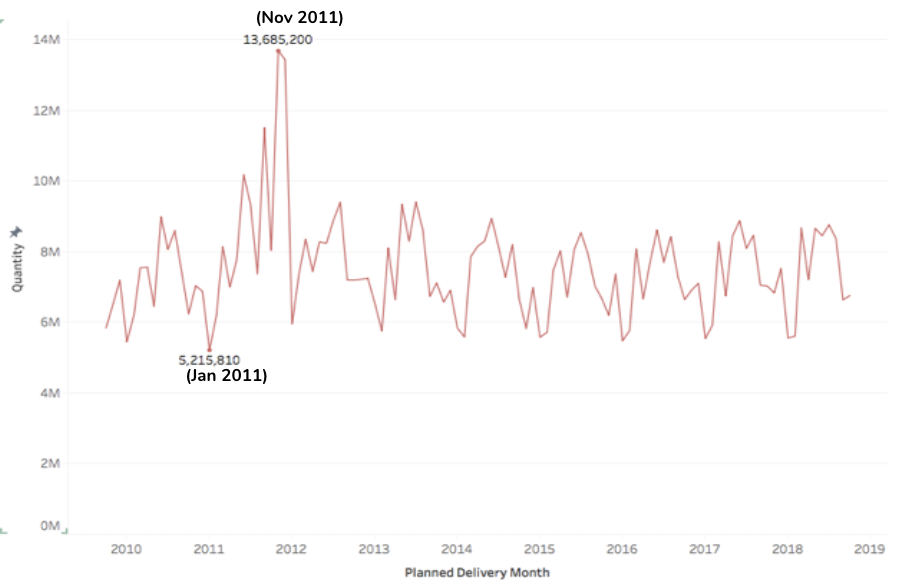
\includegraphics[width=200px,angle = 0, scale=1.5]{figure/TSCoke} 

}

\caption{Monthly Coca-Cola Bag Orders Time-series Plot}\label{fig:TSCoke}
\end{figure}
Above is a time plot of monthly Coca-Cola syrup bag orders from October 2009 to October 2019. At a glance, we observe an annual seasonal pattern with no consistent trend over time. Overall, the bag quantity orders show a mean of 7,521,158 per month. Expectedly, Scholle IPN experience the highest volume of Coca-Cola bag orders during summer months (June-August) with averages over eight million ordered bags. The only other month with an average of over eight million Coca-Cola bags is during the month of March.
\begin{figure}

{\centering 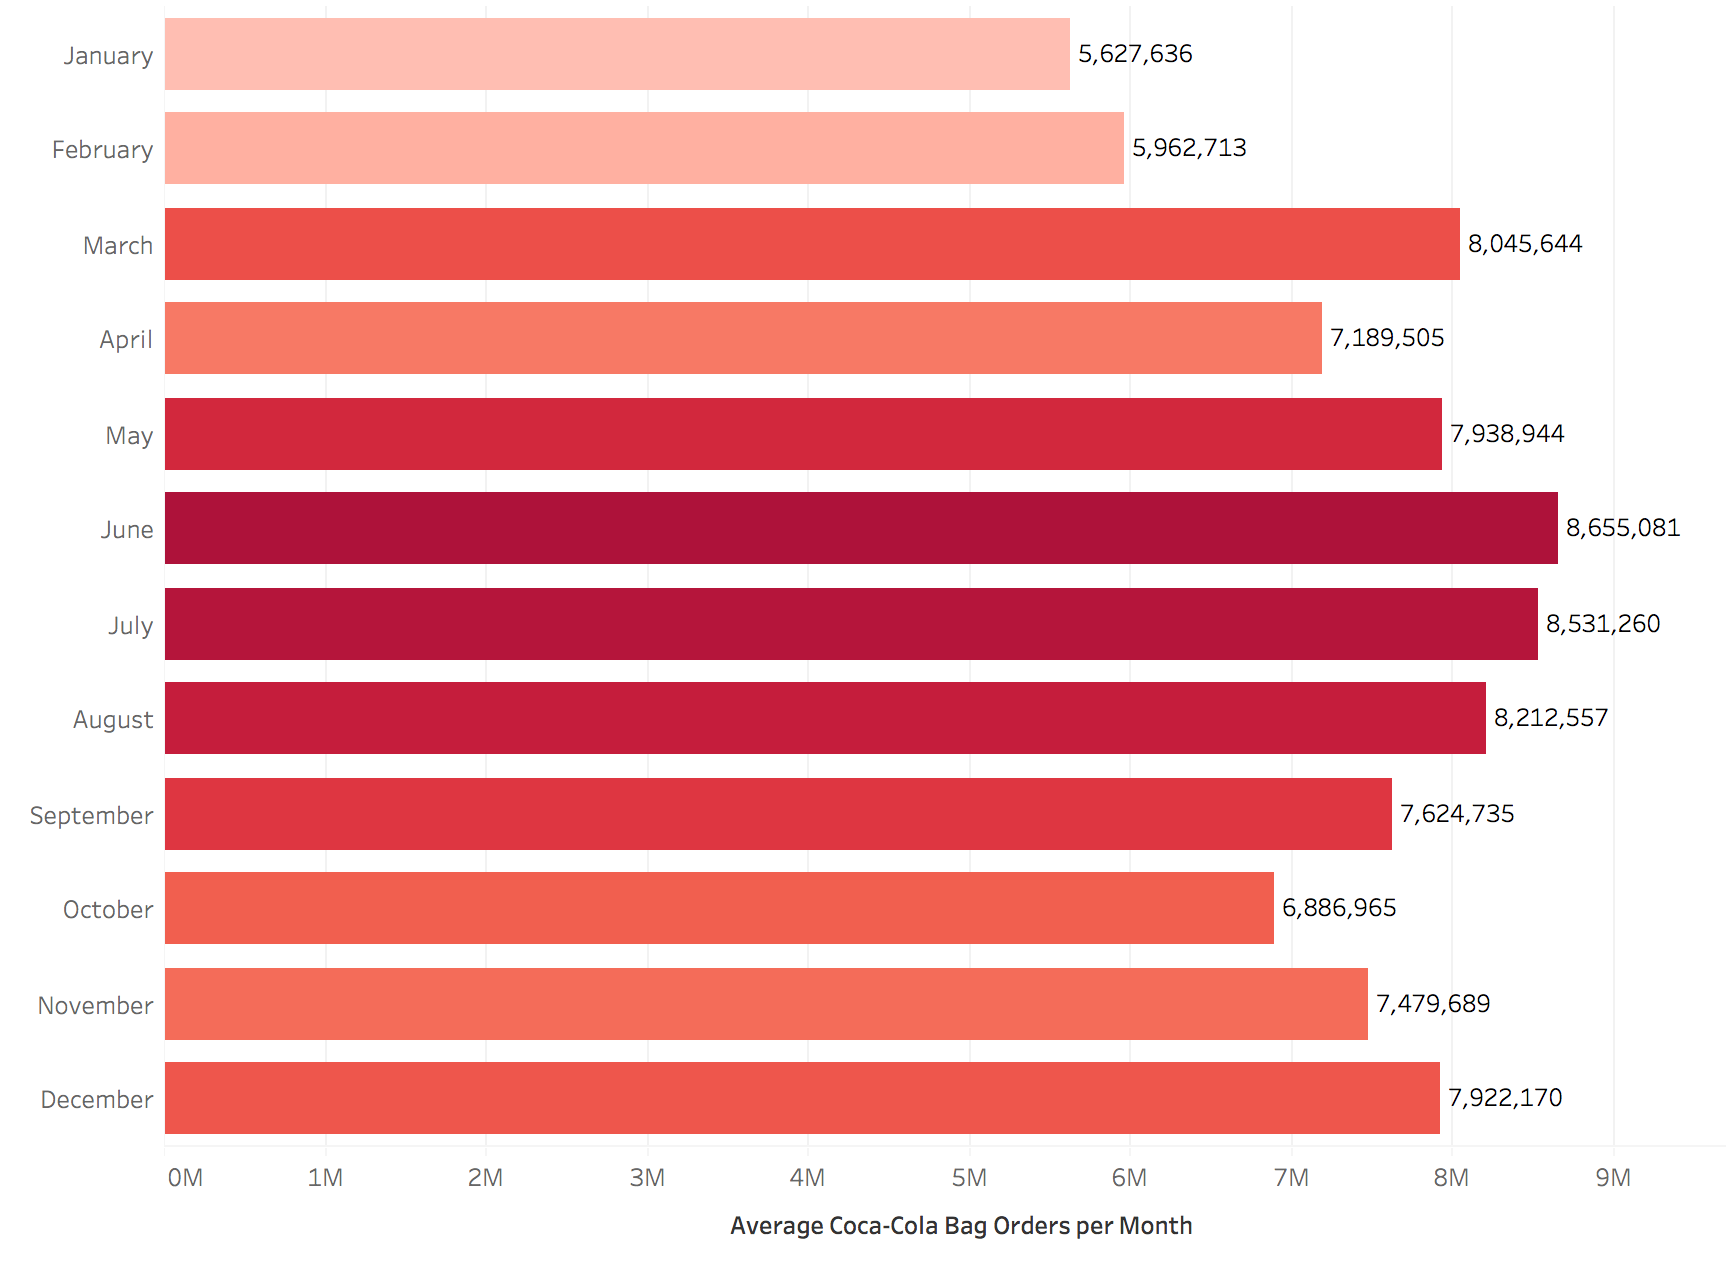
\includegraphics[width=200px,angle = 0, scale=1.5]{figure/AveCokeBagOrderPerMonth} 

}

\caption{Average Coca-Cola Bag Orders by Month}\label{fig:AveCokeBagOrderPerMonth}
\end{figure}
\hypertarget{user-generated-tweets}{%
\subsection*{User-generated Tweets}\label{user-generated-tweets}}
\addcontentsline{toc}{subsection}{User-generated Tweets}

User-generated tweets provides our forecasting models with information regarding how frequently Twitter users talk about Coca-Cola, Pepsi, McDonald's, Taco Bell, and ``jobs''. When looking at the average monthly tweet mentions for each term, the term ``jobs'' surprisingly appeared the most. Jobs-related tweets in the dataset represent 42.7\% of all the user-generated tweets collected. The visual below of the average monthly tweet volume for each selected term demonstrates how ``jobs'' represented the majority of the collected user-level data.
\begin{figure}

{\centering 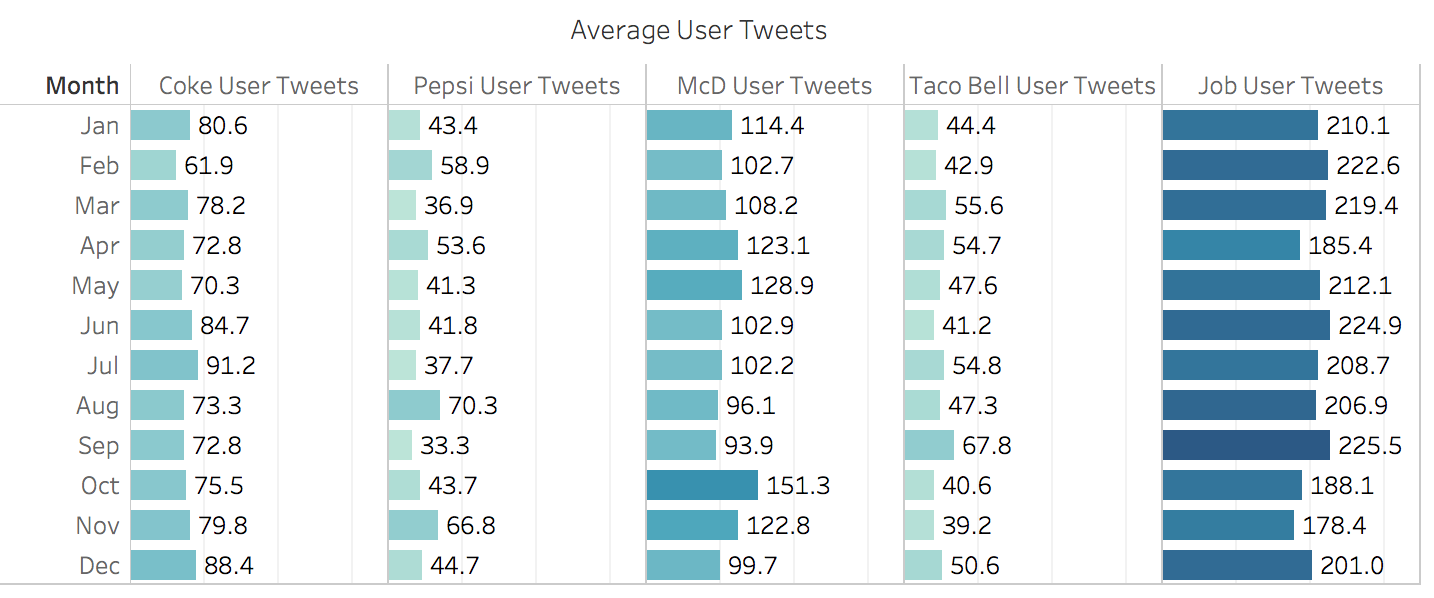
\includegraphics[width=200px,angle = 0, scale=2.1]{figure/AveUserTweets} 

}

\caption{Average User tweets by month}\label{fig:AveUserTweet}
\end{figure}
The disparity on tweet volume across topics can be explained by the limitations imposed by the Twitter Search API (please refer to the Appendix for more information). Originally, we did not anticipate the general public to engage in job-related conversation on a social media platform compared to the other relevant terms. This finding provides value to our analysis as the term ``jobs'' has a large sample size. This can potentially give us better indication on how economic activity in North America impacts Coca-Cola bag orders. However, a lower total of user-generated tweets for all other relevant terms resulted. Limited sample size for these variables could adversely impact their ability to forecast Coca-Cola bag orders.

\hypertarget{company-generated-tweets}{%
\subsection*{Company-generated Tweets}\label{company-generated-tweets}}
\addcontentsline{toc}{subsection}{Company-generated Tweets}
\begin{verbatim}
To continue the exploration of covariates, we explore company-generated tweets.  This set of social media variables provides us information about promotional behavior for these selected companies (monthly tweets) and the subsequent consumer reaction to these promotions (monthly likes, retweets and replies).  A total of 24,442 such tweets were collected between October 2009 to October 2018.  Among the four companies, the official Twitter accounts of Coca-Cola and McDonald’s were the most active in terms of posting Twitter content.  The time series plots below (not built to scale) clearly show a general trend among all four companies.  
\end{verbatim}
\begin{figure}

{\centering 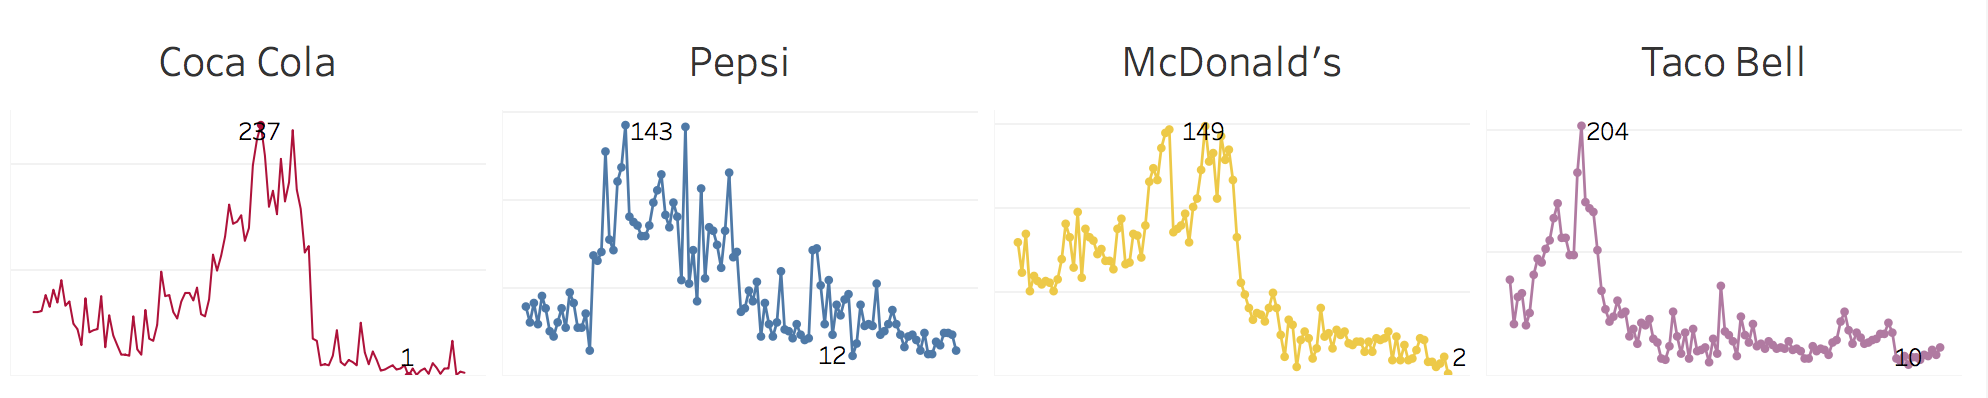
\includegraphics[width=200px,angle = 0, scale=2.1]{figure/CompanyTweets} 

}

\caption{Company Tweet Volume Time-series Plot}\label{fig:CompanyTweets}
\end{figure}
For each company, the total number of tweets per month were low in the beginning portion of the time plot. This was followed by a surge in tweet volume in the middle part of the decade suggesting how all four companies started to heavily utilize Twitter as a promotional tool. This change in behavior from companies could be attributed to the increased use of Twitter by social media consumers around the same time. The time plots below (not built to scale) of total consumer reactions (replies, likes, retweets) is a representation of how Twitter users who engaged with each company reacted to their tweets over time.
\begin{figure}

{\centering 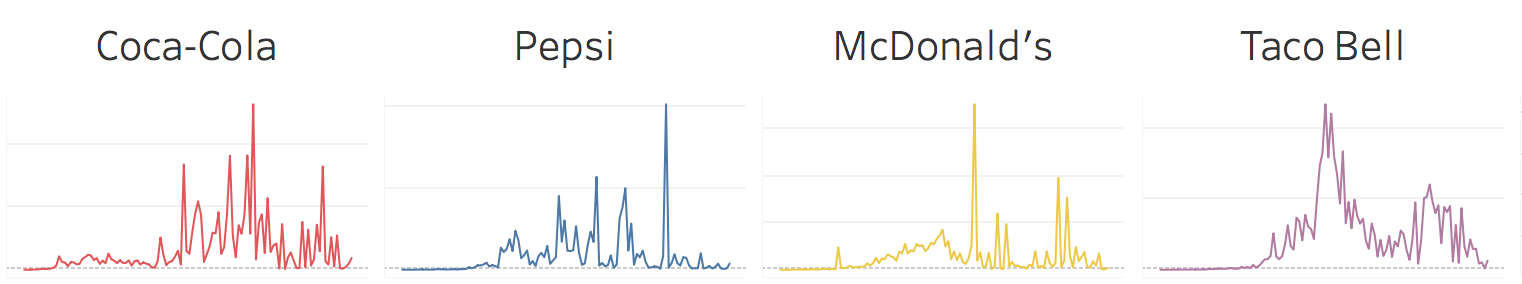
\includegraphics[width=200px,angle = 0, scale=2.1]{figure/ConsumerReactionTweets} 

}

\caption{Company Tweet Reaction (Likes, Replies, Retweets) Time-series Plot}\label{fig:ConsumerReactionTweets}
\end{figure}
Noticeably, Twitter users became much more engaged with these Twitter accounts towards the middle portion of the time plots. This could be a sign of how effective these company's promotions are during the middle of the decade, or it could be an indicator of when social media started becoming more popular in mainstream society. The limited Twitter activity by the Twitter accounts and users during the earlier portion of the time plots should be considered when modeling.

\hypertarget{google-trends}{%
\subsection*{Google Trends}\label{google-trends}}
\addcontentsline{toc}{subsection}{Google Trends}

Although Google Trends is not a social media platform, it does provide an easily attainable source of data regarding general interest in Coca-Cola, Pepsi, McDonald's, Taco Bell, and `jobs'. This could provide useful information when forecasting Coca-Cola bag orders.
Above are time series plots for each term and their monthly Google Trend value from October 2009 to October 2018. Generally, there seems to be a seasonal trend that appear for each search term. It is interesting to note that the two quick service restaurants, McDonald's and Taco Bell, experienced an increasing trend over time.
\begin{figure}

{\centering 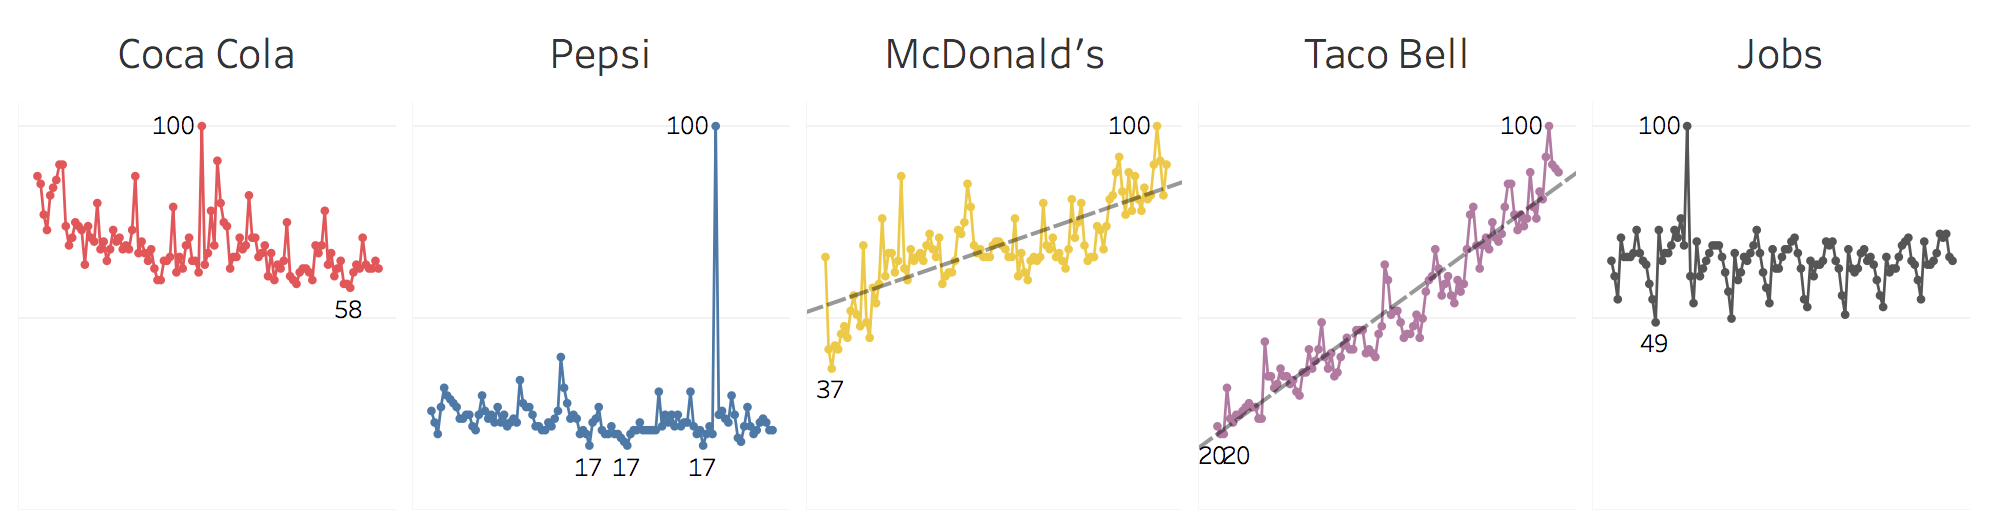
\includegraphics[width=200px,angle = 0, scale=2.1]{figure/GoogleTrends} 

}

\caption{Google Trends (by topic) Time-series Plot}\label{fig:GoogleTrends}
\end{figure}
When using Google Trends, it is important to consider that trend values are calculated strictly based on the search term entered. This strict rule could fail in certain instances where a single term could have different meanings. For example, an unusual spike can be observed in the time series plot for `jobs' in October 2011. After conducting additional research, this spike can be attributed to a sudden interest in Steve Jobs when he passed away. For Pepsi, a spike in April 2017 was traced back due to its connection to a controversial advertisement involving the celebrity Kendall Jenner. These outliers are imputed with a value that fit the distribution of the rest of the dataset.

\newpage

\hypertarget{modeling-framework}{%
\section*{Modeling Framework}\label{modeling-framework}}
\addcontentsline{toc}{section}{Modeling Framework}

\textbf{Metrics}

The following metrics are used to measure the forecasting models built using social media variables.
\begin{itemize}
\item
  Symmetric Mean Absolute Percent Error (sMAPE) - A measure based on percentage (or relative) errors.
\item
  Root Mean Square Error (RMSE) - Standard deviation of the mean squared error.
\item
  Mean Accuracy - Measures the forecast accuracy.
\item
  Percentage (\%) Bias - Measures the percentage of times the dependent variable was over- or under-estimated.
\end{itemize}
\textbf{Selection of Forecasting Models}

In this section, we describe the forecasting models used to determine if social media variables have any impact Coca-Cola bag order forecasts. We will build three types of models - baseline model, challenger models, and ensemble model. Each forecasting model is set to have a forecasting window of 18 months. The baseline model is a forecasting model using only the monthly Coca-Cola bag orders. The challenger models is a set of three different forecasting models that utilizes the social media variables. The ensemble model is a model that combines all three challenger models.

The baseline model is used to compare how challenger models that utilize social media data fare against a forecasting model that does not utilize this additional data. The baseline model is built by using a seasonal Arima model. A sliding-window cross validation of two-years, four-years, and six-years is used to determine the optimal number of observations used for training the rest of our models.

The challenger models selected for this project are: Regression with Arima errors, XGBoost, and Long Short-Term Memory (LSTM). Each challenger model is trained using 48 months of training observations (see Baseline Model Results). In addition, each challenger model will be trained on two sets of social media variables. The first set of social media variables are the difference variables identified to be cross-correlated with Coca-Cola bag orders (see Dimension Reduction section). The second set of of social media variables are the principal components identified to be cross-correlated with Coca-Cola bag orders (see Dimension Reduction section). The Regression with Arima errors assumes that Coca-Cola bag sales does not only depend on the dependent variable, but also depend on external variables selected (Hyndman, 2018). The XGBoost model is a more complex `regularized boosting' technique that seeks a good bias-variance tradeoff to reduce overfitting. It allows cross-validation at each iteration of the boosting process and thus it is easy to get the exact optimum number of boosting iterations in a single run (Chen, 2016). The final challenger model, LSTM, is a special kind of recurrent neural network that is capable of learning long-term dependencies by using adaptive, non-linear gates to update cell state information (Hochreiter, 1997). This model LSTM selectively chooses what it ``remembers'', and what to ``forget.'' In addition, LSTM selects how much of its memory it should output.
The next model used is ensemble model of all three challenger models. We compare how the challenger models and ensemble model perform against the baseline model using the metrics defined in the previous section. Furthermore, Scholle IPN is hosting other researchers from the University of Chicago to predict Coca-Cola bag orders using other external variables. The two other research teams are using related products data and economic/demographic data. The best models from these two research teams will be ensembled with the best performing social media model.

\hypertarget{scholle-system-integration}{%
\section*{Scholle System Integration}\label{scholle-system-integration}}
\addcontentsline{toc}{section}{Scholle System Integration}

\hypertarget{scholle-forecasting-model-monitoring}{%
\section*{Scholle Forecasting Model Monitoring}\label{scholle-forecasting-model-monitoring}}
\addcontentsline{toc}{section}{Scholle Forecasting Model Monitoring}

\hypertarget{findings}{%
\chapter*{Findings}\label{findings}}
\addcontentsline{toc}{chapter}{Findings}

\hypertarget{baseline-model-results}{%
\section*{Baseline Model Results}\label{baseline-model-results}}
\addcontentsline{toc}{section}{Baseline Model Results}

Before we test for the impact of social media variables in forecasting Coca-Cola bag orders, we must first establish baseline metrics. We will use a seasonal Arima model that uses only the dependent variable to establish our baseline model. Our analysis found that the best seasonal Arima model had an order of (3,0,1)(1,0,0){[}12{]}. Implementing cross validation with a sliding window of two-years, four-years, and six-years was then conducted. The purpose of cross validation is to establish the metric that the challenger models will be compared against and to find the point in the forecast horizon in which the predictions ``flatten out''. The chart below is a plot of the forecast horizon against each model's sMAPE values.
\begin{figure}

{\centering 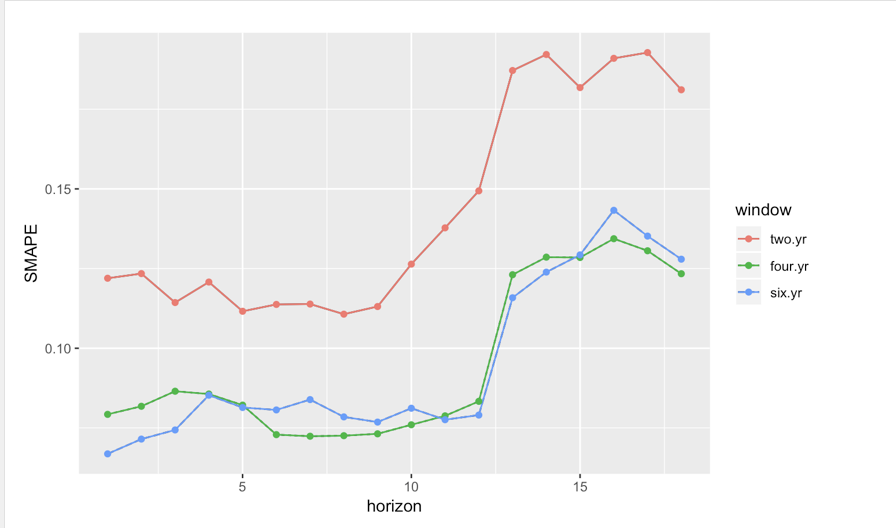
\includegraphics[width=200px,angle = 0, scale=2.1]{figure/SMAPEvsHorizon} 

}

\caption{sMAPE vs. Horizon Plot}\label{fig:SMAPEvsHorizon}
\end{figure}
It is clear that the two-year window model is considerably worse than either the four-year and six-year sliding window models. When you look at a plot of each model against the average sMAPE value for each forecast window, you can observe that the sMAPE values flatten out at the four year mark. There is no considerable improvement in sMAPE values between the four-year window model and the six-year window mode. Therefore, the best baseline model is the four-year sliding window model.
\begin{longtable}[]{@{}ccccc@{}}
\toprule
\begin{minipage}[b]{0.22\columnwidth}\centering
Sliding Window\strut
\end{minipage} & \begin{minipage}[b]{0.16\columnwidth}\centering
sMAPE\strut
\end{minipage} & \begin{minipage}[b]{0.15\columnwidth}\centering
RMSE\strut
\end{minipage} & \begin{minipage}[b]{0.16\columnwidth}\centering
Mean Accuracy\strut
\end{minipage} & \begin{minipage}[b]{0.17\columnwidth}\centering
Bias (\%)\strut
\end{minipage}\tabularnewline
\midrule
\endhead
\begin{minipage}[t]{0.22\columnwidth}\centering
2 Year\strut
\end{minipage} & \begin{minipage}[t]{0.16\columnwidth}\centering
12.79\%\strut
\end{minipage} & \begin{minipage}[t]{0.15\columnwidth}\centering
1,066,599\strut
\end{minipage} & \begin{minipage}[t]{0.16\columnwidth}\centering
86.56\%\strut
\end{minipage} & \begin{minipage}[t]{0.17\columnwidth}\centering
50.00\%\strut
\end{minipage}\tabularnewline
\begin{minipage}[t]{0.22\columnwidth}\centering
4 Year\strut
\end{minipage} & \begin{minipage}[t]{0.16\columnwidth}\centering
13.93\%\strut
\end{minipage} & \begin{minipage}[t]{0.15\columnwidth}\centering
1,215,263\strut
\end{minipage} & \begin{minipage}[t]{0.16\columnwidth}\centering
86.64\%\strut
\end{minipage} & \begin{minipage}[t]{0.17\columnwidth}\centering
38.89\%\strut
\end{minipage}\tabularnewline
\begin{minipage}[t]{0.22\columnwidth}\centering
6 Year\strut
\end{minipage} & \begin{minipage}[t]{0.16\columnwidth}\centering
14.14\%\strut
\end{minipage} & \begin{minipage}[t]{0.15\columnwidth}\centering
1,066,599\strut
\end{minipage} & \begin{minipage}[t]{0.16\columnwidth}\centering
86.49\%\strut
\end{minipage} & \begin{minipage}[t]{0.17\columnwidth}\centering
38.89\%\strut
\end{minipage}\tabularnewline
\bottomrule
\end{longtable}
\hypertarget{regression-with-arima-errors-results}{%
\section*{Regression with ARIMA Errors Results}\label{regression-with-arima-errors-results}}
\addcontentsline{toc}{section}{Regression with ARIMA Errors Results}

By evaluating the residuals and metrics, we found that regression with Arima errors produced the best results using the lagged principal components. With a sMAPE value of 9.76\% and RMSE value of 888,544, which is an improvement compared to the Scholle Coca-Cola baseline model.
\begin{longtable}[]{@{}lcccc@{}}
\toprule
\begin{minipage}[b]{0.27\columnwidth}\raggedright
Social Media Variable\strut
\end{minipage} & \begin{minipage}[b]{0.13\columnwidth}\centering
sMAPE\strut
\end{minipage} & \begin{minipage}[b]{0.14\columnwidth}\centering
RMSE\strut
\end{minipage} & \begin{minipage}[b]{0.16\columnwidth}\centering
Mean Accuracy\strut
\end{minipage} & \begin{minipage}[b]{0.16\columnwidth}\centering
Bias (\%)\strut
\end{minipage}\tabularnewline
\midrule
\endhead
\begin{minipage}[t]{0.27\columnwidth}\raggedright
Lagged Principal Components\strut
\end{minipage} & \begin{minipage}[t]{0.13\columnwidth}\centering
9.76\%\strut
\end{minipage} & \begin{minipage}[t]{0.14\columnwidth}\centering
888,544\strut
\end{minipage} & \begin{minipage}[t]{0.16\columnwidth}\centering
90.20\%\strut
\end{minipage} & \begin{minipage}[t]{0.16\columnwidth}\centering
33.00\%\strut
\end{minipage}\tabularnewline
\bottomrule
\end{longtable}
\hypertarget{xgboost-results}{%
\section*{XGBoost Results}\label{xgboost-results}}
\addcontentsline{toc}{section}{XGBoost Results}

For the XGBoost model, we introduced a month of year variable to allow the model to learn seasonality. The XGBoost performed better using the lagged social media variables producing a sMAPE value of 6.21\% and RMSE value of 597,983, which is the best performing model.
\begin{longtable}[]{@{}lcccc@{}}
\toprule
\begin{minipage}[b]{0.27\columnwidth}\raggedright
Social Media Variable\strut
\end{minipage} & \begin{minipage}[b]{0.13\columnwidth}\centering
sMAPE\strut
\end{minipage} & \begin{minipage}[b]{0.14\columnwidth}\centering
RMSE\strut
\end{minipage} & \begin{minipage}[b]{0.16\columnwidth}\centering
Mean Accuracy\strut
\end{minipage} & \begin{minipage}[b]{0.16\columnwidth}\centering
Bias (\%)\strut
\end{minipage}\tabularnewline
\midrule
\endhead
\begin{minipage}[t]{0.27\columnwidth}\raggedright
Lagged Differenced Variables\strut
\end{minipage} & \begin{minipage}[t]{0.13\columnwidth}\centering
6.21\%\strut
\end{minipage} & \begin{minipage}[t]{0.14\columnwidth}\centering
597,983\strut
\end{minipage} & \begin{minipage}[t]{0.16\columnwidth}\centering
93.88\%\strut
\end{minipage} & \begin{minipage}[t]{0.16\columnwidth}\centering
27.78\%\strut
\end{minipage}\tabularnewline
\bottomrule
\end{longtable}
After running the model, we are able to rank the features based on importance (see below).
\begin{figure}

{\centering 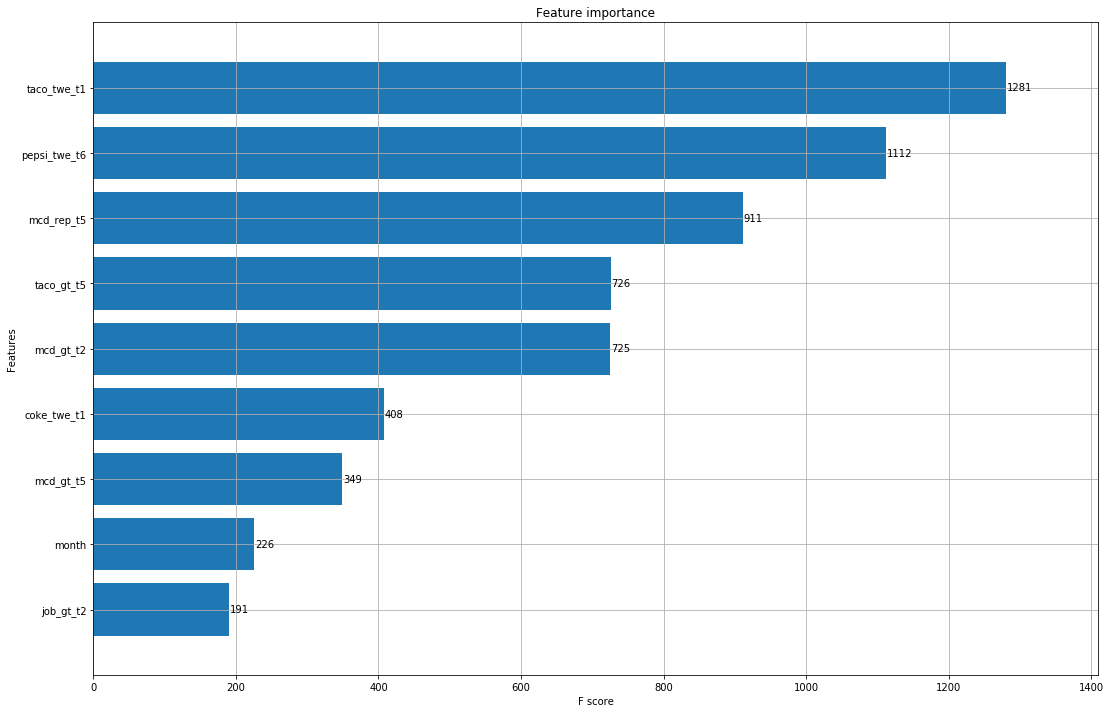
\includegraphics[width=200px,angle = 0, scale=2.1]{figure/FeatureImportance} 

}

\caption{XGBoost Feature Importance}\label{fig:FeatureImportance}
\end{figure}
\hypertarget{long-short-term-memory-results}{%
\section*{Long Short-Term Memory Results}\label{long-short-term-memory-results}}
\addcontentsline{toc}{section}{Long Short-Term Memory Results}

For the LSTM model, we also introduced a month of year variable to allow the model to learn seasonality. This model also performed better using the lagged social media variables producing a sMAPE value of 12.3\% and RMSE value of 1,023,904. This is the worst performing challenger model.
\begin{figure}

{\centering 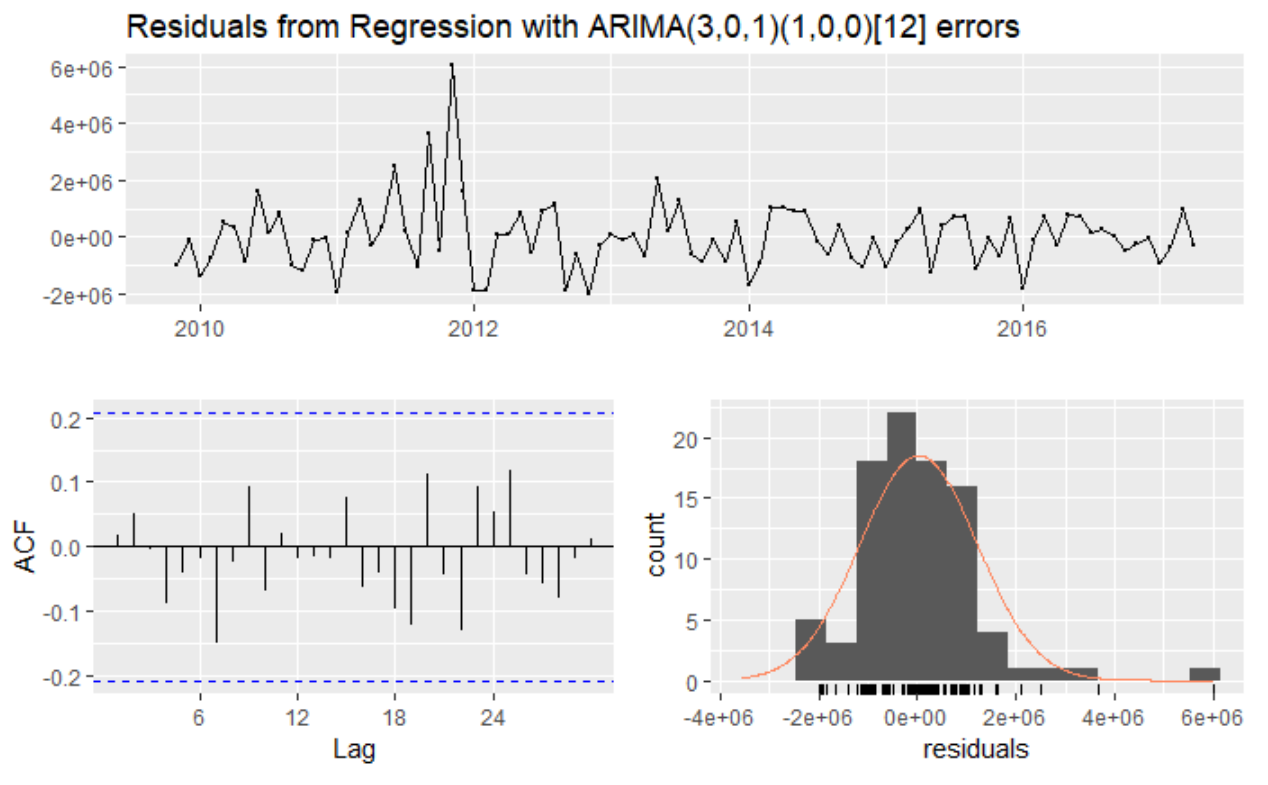
\includegraphics[width=200px,angle = 0, scale=1.5]{figure/image17} 

}

\caption{LSTM Epoch vs. Loss Function}\label{fig:image17}
\end{figure}
\begin{longtable}[]{@{}ccccc@{}}
\toprule
\begin{minipage}[b]{0.27\columnwidth}\centering
Social Media Var\strut
\end{minipage} & \begin{minipage}[b]{0.13\columnwidth}\centering
sMAPE\strut
\end{minipage} & \begin{minipage}[b]{0.14\columnwidth}\centering
RMSE\strut
\end{minipage} & \begin{minipage}[b]{0.16\columnwidth}\centering
Mean Accuracy\strut
\end{minipage} & \begin{minipage}[b]{0.16\columnwidth}\centering
Bias (\%)\strut
\end{minipage}\tabularnewline
\midrule
\endhead
\begin{minipage}[t]{0.27\columnwidth}\centering
Lagged Differenced Variables\strut
\end{minipage} & \begin{minipage}[t]{0.13\columnwidth}\centering
12.3\%\strut
\end{minipage} & \begin{minipage}[t]{0.14\columnwidth}\centering
1,023,904\strut
\end{minipage} & \begin{minipage}[t]{0.16\columnwidth}\centering
87.56\%\strut
\end{minipage} & \begin{minipage}[t]{0.16\columnwidth}\centering
38.0\%\strut
\end{minipage}\tabularnewline
\bottomrule
\end{longtable}
\hypertarget{ensemble-model-results}{%
\section*{Ensemble Model Results}\label{ensemble-model-results}}
\addcontentsline{toc}{section}{Ensemble Model Results}

After building challenger models that utilize social media variables, we will now construct an ensemble model. Wel use several ensemble models and compare these results against each individual challenger model. The ensemble models we will build are `average of all models', linear regression, and random forest.

The average of all predictions ensemble model is the most interpretable of all the ensemble models as it simply takes the average of all predicted values among all challenger models. Meanwhile, the linear model ensemble model will assign a weight to each challenger model's results. The more that a model contributes to the predicted results, the more weight the linear model will assign it. Finally, the random forest ensemble model is the most complex among the three. This model will capture how each challenger model's specific weaknesses are in prediction. For the linear regression and random forest models, the predictions of the three challenger models will be used as training observations.
\begin{longtable}[]{@{}ccccc@{}}
\toprule
\begin{minipage}[b]{0.27\columnwidth}\centering
Model\strut
\end{minipage} & \begin{minipage}[b]{0.13\columnwidth}\centering
sMAPE\strut
\end{minipage} & \begin{minipage}[b]{0.14\columnwidth}\centering
RMSE\strut
\end{minipage} & \begin{minipage}[b]{0.16\columnwidth}\centering
Mean Accuracy\strut
\end{minipage} & \begin{minipage}[b]{0.16\columnwidth}\centering
Bias (\%)\strut
\end{minipage}\tabularnewline
\midrule
\endhead
\begin{minipage}[t]{0.27\columnwidth}\centering
Scholle Baseline Model\strut
\end{minipage} & \begin{minipage}[t]{0.13\columnwidth}\centering
7.43\%\strut
\end{minipage} & \begin{minipage}[t]{0.14\columnwidth}\centering
667,832\strut
\end{minipage} & \begin{minipage}[t]{0.16\columnwidth}\centering
92.84\%\strut
\end{minipage} & \begin{minipage}[t]{0.16\columnwidth}\centering
27.78\%\strut
\end{minipage}\tabularnewline
\begin{minipage}[t]{0.27\columnwidth}\centering
Linear Regression\strut
\end{minipage} & \begin{minipage}[t]{0.13\columnwidth}\centering
5.82\%\strut
\end{minipage} & \begin{minipage}[t]{0.14\columnwidth}\centering
541,989\strut
\end{minipage} & \begin{minipage}[t]{0.16\columnwidth}\centering
94.17\%\strut
\end{minipage} & \begin{minipage}[t]{0.16\columnwidth}\centering
55.00\%\strut
\end{minipage}\tabularnewline
\bottomrule
\end{longtable}
Ensembling the three challenger models we built produced more accurate Coca-Cola bag order predictions. The results show that the random forest ensemble model performs the best according to the sMAPE and RMSE metrics. However, since the linear model produced the most stable results, this will be selected as the champion model. Below is a graph visualizing our individual model forecasts against the actual quantity (black).
\begin{figure}

{\centering 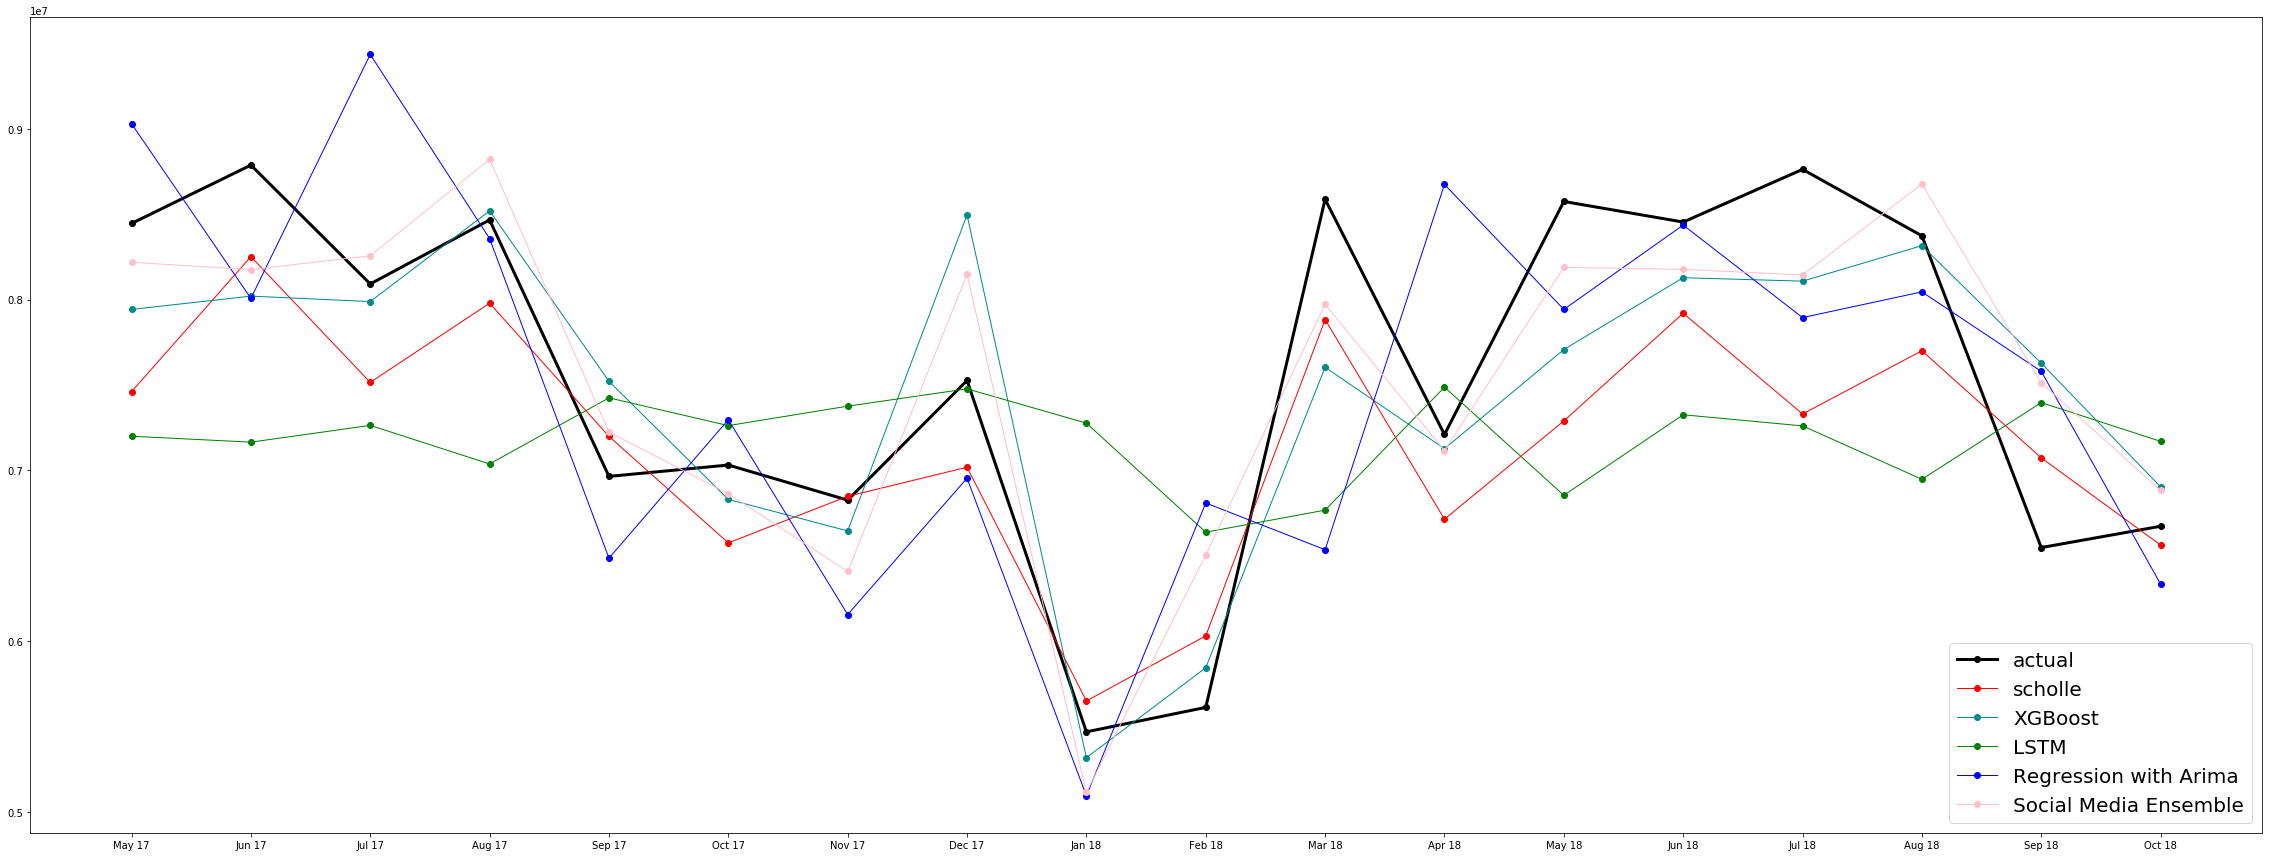
\includegraphics[width=200px,angle = 0, scale=2.5]{figure/timeplot} 

}

\caption{Model Predictions vs. Forecast Window}\label{fig:timeplot}
\end{figure}
\hypertarget{coca-cola-ensemble-model-results}{%
\section*{Coca-Cola Ensemble Model Results}\label{coca-cola-ensemble-model-results}}
\addcontentsline{toc}{section}{Coca-Cola Ensemble Model Results}

To further demonstrate the strength of ensemble modeling, this method was also used to combine models generated by other Scholle IPN capstone teams. Other teams were solving the same business problem by using a different set of covariates (related products and economy). The idea is that ensembling all the team's models will compensate for each model's weaknesses and produce a strong overall model. The final model generated incremental gains from our best ensemble model. The results are outlined below.
\begin{longtable}[]{@{}ccccc@{}}
\toprule
\begin{minipage}[b]{0.27\columnwidth}\centering
Model\strut
\end{minipage} & \begin{minipage}[b]{0.13\columnwidth}\centering
sMAPE\strut
\end{minipage} & \begin{minipage}[b]{0.14\columnwidth}\centering
RMSE\strut
\end{minipage} & \begin{minipage}[b]{0.16\columnwidth}\centering
Mean Accuracy\strut
\end{minipage} & \begin{minipage}[b]{0.16\columnwidth}\centering
Bias (\%)\strut
\end{minipage}\tabularnewline
\midrule
\endhead
\begin{minipage}[t]{0.27\columnwidth}\centering
Scholle Baseline Model\strut
\end{minipage} & \begin{minipage}[t]{0.13\columnwidth}\centering
7.43\%\strut
\end{minipage} & \begin{minipage}[t]{0.14\columnwidth}\centering
667,832\strut
\end{minipage} & \begin{minipage}[t]{0.16\columnwidth}\centering
92.84\%\strut
\end{minipage} & \begin{minipage}[t]{0.16\columnwidth}\centering
27.78\%\strut
\end{minipage}\tabularnewline
\begin{minipage}[t]{0.27\columnwidth}\centering
Linear Regression (social media)\strut
\end{minipage} & \begin{minipage}[t]{0.13\columnwidth}\centering
5.76\%\strut
\end{minipage} & \begin{minipage}[t]{0.14\columnwidth}\centering
545,211\strut
\end{minipage} & \begin{minipage}[t]{0.16\columnwidth}\centering
94.22\%\strut
\end{minipage} & \begin{minipage}[t]{0.16\columnwidth}\centering
50.00\%\strut
\end{minipage}\tabularnewline
\begin{minipage}[t]{0.27\columnwidth}\centering
Linear Regression\strut
\end{minipage} & \begin{minipage}[t]{0.13\columnwidth}\centering
1.05\%\strut
\end{minipage} & \begin{minipage}[t]{0.14\columnwidth}\centering
93,662\strut
\end{minipage} & \begin{minipage}[t]{0.16\columnwidth}\centering
98.95\%\strut
\end{minipage} & \begin{minipage}[t]{0.16\columnwidth}\centering
44.44\%\strut
\end{minipage}\tabularnewline
\begin{minipage}[t]{0.27\columnwidth}\centering
Random Forest\strut
\end{minipage} & \begin{minipage}[t]{0.13\columnwidth}\centering
1.34\%\strut
\end{minipage} & \begin{minipage}[t]{0.14\columnwidth}\centering
119,437\strut
\end{minipage} & \begin{minipage}[t]{0.16\columnwidth}\centering
98.64\%\strut
\end{minipage} & \begin{minipage}[t]{0.16\columnwidth}\centering
50.00\%\strut
\end{minipage}\tabularnewline
\bottomrule
\end{longtable}
\begin{figure}

{\centering 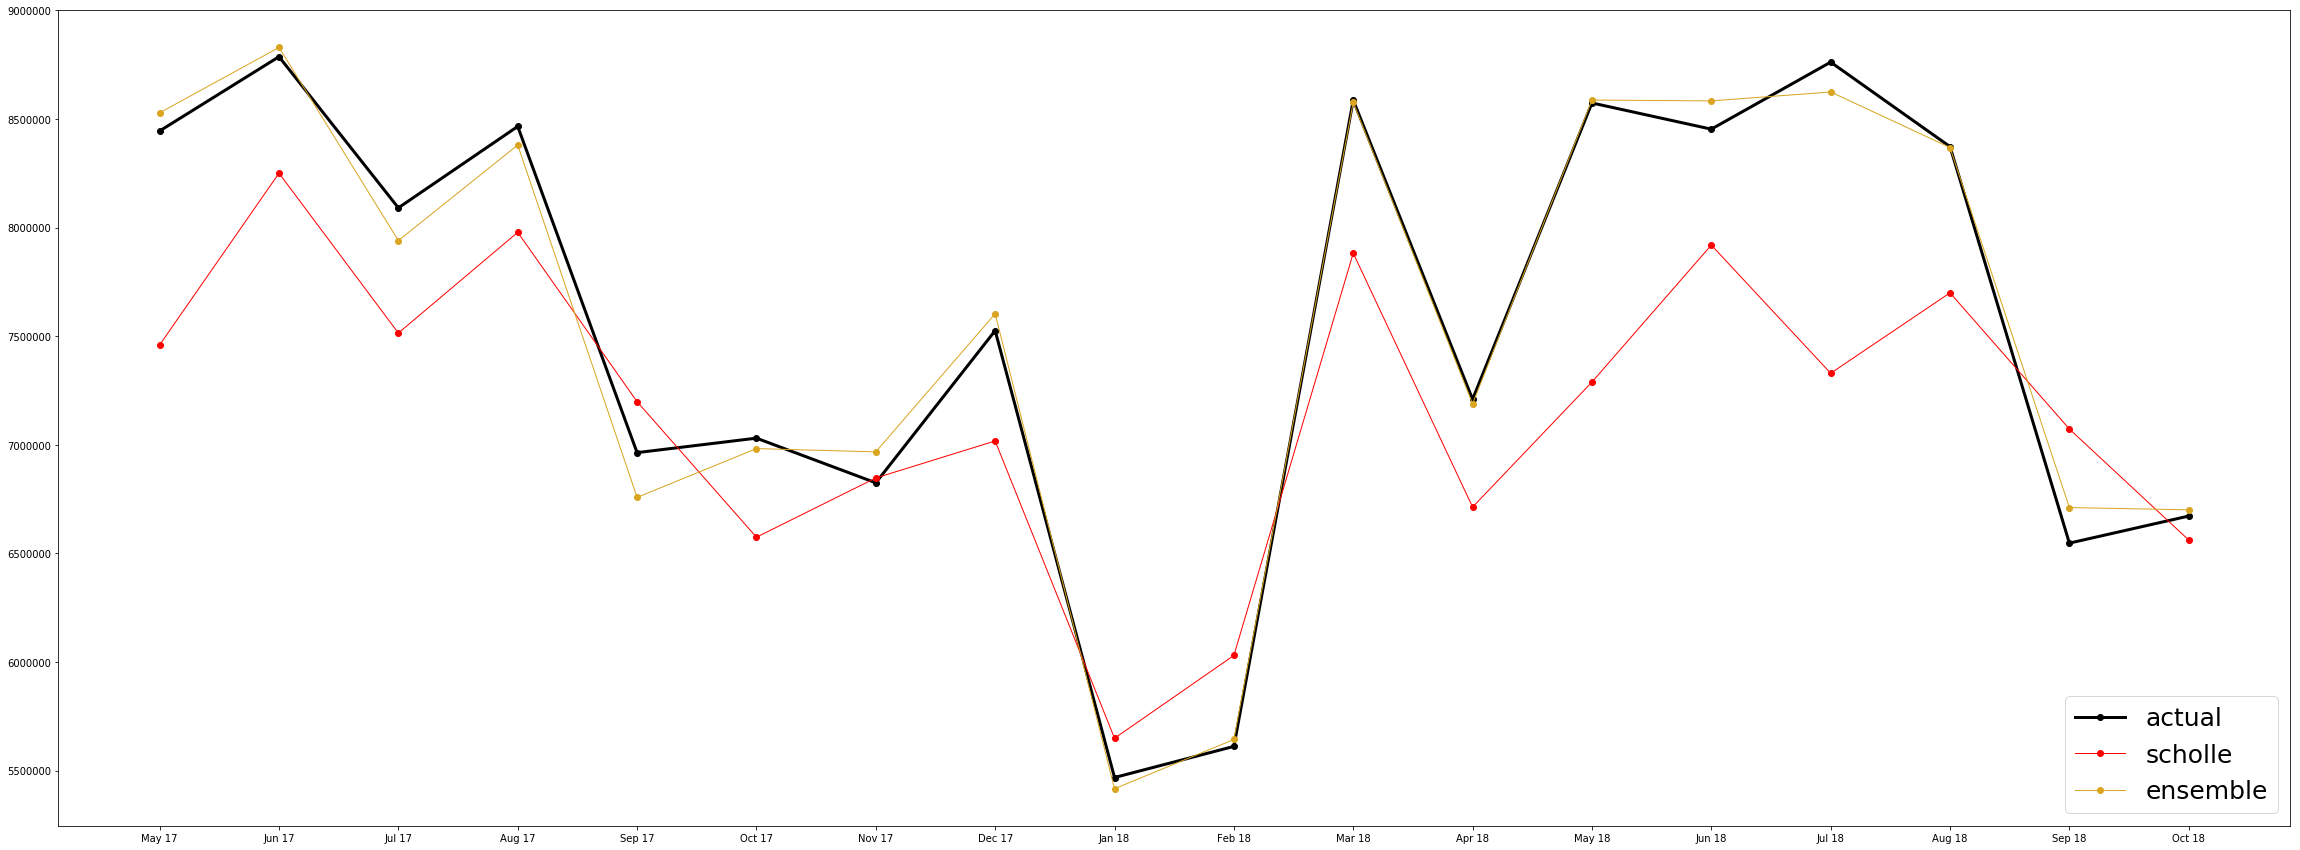
\includegraphics[width=200px,angle = 0, scale=2.5]{figure/coketeams} 

}

\caption{Coke Ensemble Model Predictions vs. Forecast Window}\label{fig:coketeams}
\end{figure}
\hypertarget{conclusion}{%
\chapter*{Conclusion}\label{conclusion}}
\addcontentsline{toc}{chapter}{Conclusion}

In summary, we learned that social media variables improved Scholle IPN's forecsts of Coca-Cola bag orders. Even though sentiment analysis is an effective way of converting textual social media data into numerical data, we found that sentiment scores is largely dependent upon the text data available. Our user tweet data was not evenly distributed leading to a biased average sentiment score for each topic. This rendered these variables to be inconclusive for predicting Coca-Cola bag orders. Additionally, identifying the social media variables that were cross-correlated with Coca-Cola bag orders were found to improve the XGBoost and LSTM models. According to XGBoost, the most important features are Taco Bell account tweets (t-1), Pepsi account tweets (t-6), and McDonald account replies (t-5). Meanwhile, the principal component variables were effective in improving Coca-Cola bag predictions for the regression with Arima errors model. Furthermore, using an ensemble approach to modeling provides better overall results. The results for ensembling the social media challenger models (Regression with Arima errors, XGBoost, and LSTM) were considerably better than any of the individual model results. In addition, the ensemble model of the best performing models for each Scholle IPN research teams produced the best overall Coca-Cola forecasting model.

\hypertarget{recommendations}{%
\chapter*{Recommendations}\label{recommendations}}
\addcontentsline{toc}{chapter}{Recommendations}

Based on this research, our team recommends the following:
\begin{itemize}
\tightlist
\item
  Use data from the social media accounts of Coca-Cola's main competitors and top quick service restaurants for building forecasting model.
\item
  Collect more historical user-level tweets for each topic to generate a represenative average sentiment score for the forecasting model.
\end{itemize}
\hypertarget{future-work}{%
\chapter*{Future Work}\label{future-work}}
\addcontentsline{toc}{chapter}{Future Work}

For this project, we focused our data collection on only a handful of quick service restaurants and competitors. Our analysis found that the top variables related to Pepsi, Taco Bell, and McDonald's. For future work, collecting social media data from additional Coca-Cola competitors could present an opportunity to improve the existing forecasting model. Hence, it may bring better accuracy in predicting the Coca-Cola bag sales for Scholle IPN. Additionally, increasing the transparency and easiness of the models. Machine learning models carry more parameters, require more setup, and take longer steps than the current forecasting decision-making protocol. Therefore, it is essential for C-suite to fully grasp the importances of each single external variable on a more granular level. If the significance of each input is needed, we recommend to introduce Shapley Values for better interpretability, as it gives the average marginal contribution of a feature value across all possible coalitions (Molnar, 2019).

\newpage

\appendix

\hypertarget{appendix}{%
\chapter*{Appendix A}\label{appendix}}
\addcontentsline{toc}{chapter}{Appendix A}

\textbf{KPSS Test}
\url{https://www.rdocumentation.org/packages/tseries/versions/0.10-46/topics/kpss.test}
(Insert table of KPSS test results - before and after differencing)

\textbf{Data Cleansing}
Scholle IPN Data
The Scholle IPN data provides a variety of relevant data features that uninformed users can use to gain knowledge about Scholle IPN's product. Our team will use this data to find relevant trends that may be useful in forecasting. The table below describes the Scholle IPN metadata:

Prior to searching for any relevant patterns in the Scholle IPN data, it is best practice to conduct preliminary data cleansing. First, we notice that there are 8,204 total orders in this dataset ranging from a delivery date of 10/1/2009 to 11/2/2018. It is important to note that this dataset is a combination of orders from all of Scholle IPN clients in their syrup bag product line. Of all the orders, 5,118 of the records lists `Coca-Cola' as the top business partner. Other issues include null values being present for the `Ship\_to\_State' variable and negative values for `quantity' variable.

The following data cleansing steps were conducted to prepare the Scholle IPN data for monthly aggregation:
\emph{Filter syrup bag orders for `Coca-Cola' top business partner.\\
}Drop records with quantities of less than one thousand.\\
\emph{Impute records with missing values in `Ship\_to\_State' with `Bayamon, PR'.
}Drop records outside of the United States and Canada market.
*Drop records that occurred after October 2018.

Once the steps listed have been conducted, the primary data is left with only 4,875 records. The final step to data cleansing will be aggregating the records at the monthly level. The `Planned Delivery Date' field will be used to aggregate quantities at the desired level.

\textbf{Twitter Data Collection}
The selected terms (Coca-Cola, Pepsi, McDonald's, Taco Bell, Jobs) will be used to collect user-generated tweets. The collection of this data will be done by using Twitter's Search API. Twitter posts containing the terms `coke', `pepsi', `mcdonalds', `taco bell', or `jobs' will be collected from the 15th of every month from July 2009 to December 2018. Twitter's Search API impose strict restrictions on query results depending on the account level purchased. For this project, a maximum of 500 user-generated tweets will be collected per month in the given date range. For example, for the month of December 2018, there will be 500 tweets collected related to Coca-Cola, Pepsi, McDonald's, Taco Bell, and jobs. This means that at any given month, the distribution of tweets across different terms can differ depending on what search term is trending.

Since this project is concerned with the US and Canada markets, we need to add a series of Search API query constraints to ensure that collected tweets are mainly from users in these selected markets. The first constraint was to query results in the english language by filtering for user profiles with country codes of `us' or `ca'. The second constraint involves the time of day that the tweets were posted. Since Twitter Search API collects tweets in reverse chronological order given a date and time, a time constraint of 23:00 UTC (6 pm CST) was applied to the queries to ensure that collected tweets will fall in a time range when most people in the US and Canada are off normal working hours. This will provide a robust collection of tweets from a variety of different users across different regions of the US and Canada. The final output of these Twitter search queries will include the tweet content, tweet date and time, number of replies, number of retweets, and number of likes.

The second approach to collecting Twitter data is to gather historical Twitter posts generated by the official Twitter accounts of Coca-Cola, Pepsi, McDonald's, and Taco Bell from July 2009 to December 2018 using a separate web scraping tool. These selected Twitter accounts vary greatly in their online activity. While some accounts, like Taco Bell, reply frequently to their followers, other accounts tend to be less engaging and post infrequently. For the purpose of this project, only independent tweets posted by each Twitter account will be collected. This means that tweet replies to Twitter users will not be collected. The main benefit of this approach is that it allows us to focus on tweets that promote individual marketing campaigns. The final output of this data collection step will include tweet content, tweet date and time, number of replies, number of retweets, and number of likes.\\
The total output of the Twitter data collection results are 56,528 user-generated tweets and 24,442 company-generated tweets from July 2009 to December 2018. For both datasets, tweets outside of October 2009 to October 2018 will be filtered out to prepare for time series modeling.

The user-generated tweets will require additional pre-processing steps prior to monthly aggregation. The Twitter Search API collects tweets on a rule-based approach meaning it is probable that nonsensical tweets may be included in the raw data collected. For example, tweets referencing the drug `cocaine' (or `coke' in colloquial terms) were identified in the raw data. A series of natural language processing steps were conducted on the tweet's text to help screen out these ``noisy`` tweets. In addition, these steps will be important to prepare the tweet data for aggregation. Some of these processing steps include removing stopwords, creating n-grams, and tokenizing text. After conducting text processing steps, an R package was used to calculate the sentiment of a given tweet. This step will provide us with an additional feature that will inform business users about user sentiment on their product. After these pre-processing steps, the tweets will now be aggregated on a monthly level to generate the following independent variables for each search term (Coca-Cola, Pepsi, McDonald's, Taco Bell, ``Jobs''): total tweets per month, total replies per month, total likes per month, total retweets per month, and average sentiment per month. There are a total of 25 variables generated from this step.
The company-generated tweets from Coca-Cola, Pepsi, McDonald's, and Taco Bell will be aggregated on a monthly level to generate the following independent variables for each Twitter account (Coca-Cola, Pepsi, McDonald's and Taco Bell): total tweets per month, total replies per month, total likes per month, total retweets per month. There are a total 16 variables generated from this step.

\textbf{Google Trends Data}
Google Trends data will also be collected to better anticipate the demand for Coca-Cola products. Although Google Trends is not a social media platform, it does provide its users with quantified information about the relative popularity of a search term over time. The monthly Google Trend values for the following terms will be collected: Coca-Cola, Pepsi, McDonald's, Taco Bell, and `Jobs'. Each topic will be queried individually with the date range October 2009 to October 2018. Google Trend values for each term will range between 0 to 100, with 100 signifying the month in which the term was most popular. No additional preprocessing is required for Google Trends data. There are a total of five variables generated from this step.

\textbf{Exploratory Data Analysis - Scholle IPN}
The maximum quantity of bags ordered occurred in November 2011 with a total of 13,685,000 bag orders, while the minimum quantity of bags ordered occurred in January 2011 with a total of 5,215,810 bag orders. After exploring the Scholle IPN data, it was also observed that the Columbus (OH), Atlanta (GA), and Dallas (TX) are the top cities where Coca-Cola bag orders were being delivered. Given that information, it is less surprising to observe that the top three states by quantity of bag order deliveries were Ohio, Georgia, and Texas. In terms of Coca-Cola bag products, the stock-keeping unit (SKU) 200258 and 200144 were the two most ordered SKU.

\textbf{Exploratory Data Analysis - Social Media Variables}
Similar to the Scholle IPN data, it is important to explore our covariates to identify any underlying trends that could be used to forecast Coca-Cola demand. For user-generated tweets, a total of 52,952 user-generated tweets were collected between October 2009 to October 2018. Among the four companies, McDonald's is the most talked about company over the given date range. When exploring which terms appear the most with each other, the term that appeared most commonly with Coca-Cola is Pepsi.

\textbf{Sentiment Analysis}
\url{https://github.com/trinker/sentimentr}

\backmatter

\hypertarget{references}{%
\chapter*{References}\label{references}}
\addcontentsline{toc}{chapter}{References}

\markboth{References}{References}

\noindent

\setlength{\parindent}{-0.20in}
\setlength{\leftskip}{0.20in}
\setlength{\parskip}{8pt}

\hypertarget{refs}{}
\leavevmode\hypertarget{ref-angel2000}{}%
Angel, E. (2000). \emph{Interactive computer graphics : A top-down approach with opengl}. Boston, MA: Addison Wesley Longman.

\leavevmode\hypertarget{ref-angel2001}{}%
Angel, E. (2001a). \emph{Batch-file computer graphics : A bottom-up approach with quicktime}. Boston, MA: Wesley Addison Longman.

\leavevmode\hypertarget{ref-angel2002a}{}%
Angel, E. (2001b). \emph{Test second book by angel}. Boston, MA: Wesley Addison Longman.

\leavevmode\hypertarget{ref-brockwell1991}{}%
Brockwell, P. J., \& Davis, R. A. (2018). \emph{Time series: Theory and methods, 2nd edition} (pp. 373--375). Springer-Verlag, New York.

\leavevmode\hypertarget{ref-chen2016}{}%
Chen, T., \& Guestrin, C. (2016). XGBoost: A scalable tree boosting system. \emph{KDD '16 Proceedings of the 22nd ACM SIGKDD International Conference on Knowledge Discovery and Data Mining}, 785--794.

\leavevmode\hypertarget{ref-connor1994}{}%
Connor, J., Martin, R., \& Atlas, L. (1994). Recurrent neural networks and robust time series prediction. \emph{IEEE Transactions on Neural Networks}, \emph{5}(2), 240--254.

\leavevmode\hypertarget{ref-hochreiter1997}{}%
Hochreiter, S., \& Schmidhuber, J. (1997). Long short-term memory. \emph{Neural Computation}, \emph{9}(8), 1735--1780.

\leavevmode\hypertarget{ref-hyndman2018}{}%
Hyndman, R. J., \& Athanasopoulos, G. (2018). \emph{Forecasting: Principles and practice} (p. Section 9.2). Melbourne, Australia: OTexts.

\leavevmode\hypertarget{ref-kambhatla1997}{}%
Kambhatla, N., \& Leen, T. K. (1997). Dimension reduction by local principal component analysis. \emph{Neural Computation}, 1493--1516. Retrieved from \href{https://doi.org/10.1162/neco.1997.9.7.1493\%20}{https://doi.org/10.1162/neco.1997.9.7.1493 }

\leavevmode\hypertarget{ref-kwiatkowski1992}{}%
Kwiatkowski, D., Peter Schmidt, P. C. P. snd, \& YongcheolShin. (1992). Testing the null hypothesis of stationarity against the alternative of a unit root: How sure are we that economic time series have a unit root? \emph{Journal of Econometrics}, 159--178. Retrieved from \url{https://doi.org/10.1016/0304-4076(92)90104-Y}

\leavevmode\hypertarget{ref-molnar2019}{}%
Molnar, C. (2019). \emph{Interpretable machine learning - a guide for making black box models explainable} (pp. Chapter 5, Section8). Springer-Verlag, New York.

\leavevmode\hypertarget{ref-pavlyshenko2019}{}%
Pavlyshenko, B. M. (2019). Machine-learning models for sales time series forecasting. \emph{MDPI}. Retrieved from \url{https://www.mdpi.com/2306-5729/4/1/15/pdf}

\leavevmode\hypertarget{ref-shi2015}{}%
Shi, X., Chen, Z., Wang, H., Yeung, D.-Y., Wong, W.-K., \& Woo, W.-c. (2015). Convolutional lstm network: A machine learning approach for precipitation nowcasting.


% Index?

\end{document}
